\documentclass{ieeeaccess}
%Adjusted 05/13/2026 at the byline author names
% Official IEEE Access LaTeX template (ACCESS_latex_template_20260513).
% GENERATED by paper/build_latex.py from paper/sections; edit the sections,
% not this file, or your edits are lost on the next build.
\usepackage{cite}
\usepackage{amsmath,amssymb,amsfonts}
% \usepackage{algorithmic}  % not used; not in every TeX install
\usepackage{graphicx}
\usepackage{textcomp}
\usepackage{tabularx}
\usepackage{url}
\makeatletter\g@addto@macro{\UrlBreaks}{\UrlOrds}\makeatother % let long URLs break
\renewcommand{\tabularxcolumn}[1]{>{\raggedright\arraybackslash}p{#1}}

\usepackage{bm}
\makeatletter
\AtBeginDocument{\DeclareMathVersion{bold}
\SetSymbolFont{operators}{bold}{T1}{times}{b}{n}
\SetSymbolFont{NewLetters}{bold}{T1}{times}{b}{it}
\SetMathAlphabet{\mathrm}{bold}{T1}{times}{b}{n}
\SetMathAlphabet{\mathit}{bold}{T1}{times}{b}{it}
\SetMathAlphabet{\mathbf}{bold}{T1}{times}{b}{n}
\SetMathAlphabet{\mathtt}{bold}{OT1}{pcr}{b}{n}
\SetSymbolFont{symbols}{bold}{OMS}{cmsy}{b}{n}
\renewcommand\boldmath{\@nomath\boldmath\mathversion{bold}}}
\makeatother

%Your document starts from here ___________________________________________________
\begin{document}
\history{Date of publication xxxx 00, 0000, date of current version xxxx 00, 0000.}
\doi{10.1109/ACCESS.2024.0429000}

\title{An 8\% Learned Energy Saving That Was a Plant-Model Artefact: Processor-in-the-Loop Evaluation of Rule-Based and Learned Electric-Vehicle Energy Management on a Microcontroller}
\author{\uppercase{Manikanta Gonugondla}\authorrefmark{1} AND \uppercase{Swathi Tangi}\authorrefmark{1}}
\address[1]{[Affiliation to be confirmed by the authors before submission]}
\tfootnote{Funding information to be added by the authors.}

\markboth
{M. Gonugondla \headeretal: An 8\% Learned Energy Saving That Was a Plant-Model Artefact}
{M. Gonugondla \headeretal: An 8\% Learned Energy Saving That Was a Plant-Model Artefact}

\corresp{Corresponding author: Swathi Tangi (e-mail: to be added).}

\begin{abstract}
A learned electric-vehicle energy manager is trained and scored against a simulated vehicle, so a physical inconsistency in that model can be read as a gain. This paper reports one such case and the audit that exposed it. A rule-based energy manager and a Soft Actor-Critic (SAC) policy ran as a 10 Hz supervisory task on an ESP32-S3 microcontroller, above a 100 Hz speed loop, in a processor-in-the-loop (PIL) arrangement against a longitudinal vehicle model identified from logged winter trips. In a first campaign the policy appeared to cut model-computed energy by 8.28\%, using less in 14 of 16 settings, and a repeat reproduced it. The model capped billed battery power at the policy's ceiling but computed acceleration from the uncapped torque. Repetition and trip replay could not see this. It surfaced when the policy finished 7\% below a feasible dynamic-programming reference, and a controller-free sweep then drove US06 on 8.05 Wh/km at a 5 kW ceiling. After correction and retraining, the evaluated SAC design used more energy than the rules in all 12 distinct conditions, each averaged over three paired noise draws (median +0.50\%, exact Wilcoxon p = 0.0005), and tracked speed worse. The 8.28\% result is withdrawn. The checks are set out as a reusable physical-consistency audit, with tested and untested parts kept apart. Filtering the speed reading recovered the energy lost at ten times the sensor-noise floor. Absolute Wh/km figures belong to this model, whose median trip-energy error on a second vehicle is 13\% to 17\%.
\end{abstract}

\begin{keywords}
Electric vehicles, energy management, fault detection, Kalman filters, microcontrollers, processor-in-the-loop, reinforcement learning, time series forecasting
\end{keywords}

\titlepgskip=-21pt

\maketitle

\section{INTRODUCTION}
\label{sec:intro}

\PARstart{A}{} learned energy manager for a battery electric vehicle (EV) is trained against a simulated vehicle and usually scored against the same one. The policy is an optimiser, and it optimises the model as written, not the vehicle the model was meant to describe. Any path by which the model pays for an action without charging its physical cost is therefore a lever the policy can find, a pattern known in reinforcement learning as reward hacking~\cite{amodei2016}. Results in deep reinforcement learning also vary with the random seed and with how the baseline is tuned~\cite{henderson2018}, and the gap between laboratory results and deployed controllers is well documented~\cite{dulac2021}. A reported gain of a learned energy manager over a rule set is only as good as the checks that rule out the model as its source.

This paper reports a gain that did not survive those checks, and the checks that found it. The setting is a processor-in-the-loop (PIL) study. A rule-based energy manager and a Soft Actor-Critic (SAC) policy~\cite{haarnoja2018} ran on an ESP32-S3 microcontroller~\cite{esp32s3} as a supervisory task at 10 Hz, above a speed loop at 100 Hz, while a longitudinal vehicle model on a host computer exchanged state and commands with the target every 10 ms. The arrangement is PIL and not hardware-in-the-loop: the processor is real, but the motor, inverter and battery are simulated. The model was identified and validated on logged BMW i3 trips~\cite{i3data} and checked for transfer on the Vehicle Energy Dataset (VED)~\cite{ved}. The controllers ran the UDDS, HWFET and US06 drive cycles~\cite{epacycles}. Acceptance gates and pass criteria were written before each experiment; every rule or revision made after results were seen, and every run attempted, is listed in Section~\ref{sec:platform}. Each result carries one of three labels. Target-measured covers timing, counters and memory recorded on the microcontroller. PIL-evaluated covers energy, tracking and other vehicle outcomes that the host model computed while the controller ran on the target; no battery was metered. Host-simulated covers work on the host alone.

The work began from the study of Tangi et al.~\cite{tangi2025}, which predicted EV range, optimum acceleration and optimum velocity with Random Forest, Extra Trees, Linear Regression and Long Short-Term Memory models and their ensembles. That study used a synthetically generated dataset of 2,000 samples and served the trained models through a web application, and its authors named real-world data and embedded evaluation among the next steps. Three questions follow from its declared scope: whether such conclusions hold on logged trips, what happens when a learned model closes a control loop around a vehicle, and whether the chain runs on an embedded controller under a real-time deadline. The second question is where the artefact appeared.

In the first campaign on the target, the learned policy used less energy than the rules in 14 of 16 settings, by 8.28\% on average. A repeat campaign, on separately flashed firmware, gave 14 of 16 again, and the energy of the 32 settings in which both campaigns tracked the cycle agreed to 0.18\% on average. Firmware that logged the policy's battery power ceiling was added, and it showed the policy holding the ceiling lower than the rules did, which fitted the explanation then recorded as inferred: that the policy saved energy by shaving current peaks. The explanation was wrong. The vehicle model capped the battery power it billed at the ceiling but computed acceleration from the torque requested before the cap, so a low ceiling cut the energy charged and left the motion untouched. The policy had been trained on that model and had learned to use it.

None of the study's standing safeguards could see this fault. Repetition on the target reproduces whatever the model does, and timing measurements do not pass through the energy bookkeeping. Gate G2 validates the model by replaying logged trips with a ceiling that never binds. The plant's own unit test asserted that billed power met the ceiling exactly; it did not assert that the vehicle slowed. What exposed the fault was a reference computed before any policy was trained. A dynamic-programming (DP) policy~\cite{bellman1957}, run through the full model as an approximate feasible-policy reference, gave 190.39 Wh/km over the US06 cycle, and the policy reached 176.4 Wh/km on the target at the same distance and tracking error. The rules came within 0.04\% of that reference. A learned result 7\% below a feasible reference is not proof of a fault, since the reference is approximate, but it was a reason to audit, and the model came under suspicion before the policy did. The pattern of the gain agreed. It grew with demand on three independent axes and vanished on UDDS and HWFET, where demand stays below the policy's lowest ceiling of 40 kW. A sweep of fixed ceilings with no controller in the loop then settled it: at 5 kW the model drove all 12.888 km of US06 on 8.05 Wh/km with an unchanged tracking error of 0.0013 m/s (host-simulated).

After the fix, a binding ceiling takes torque away, and a test asserts that traction never exceeds what the battery supplied. A limit that does not bind leaves every output unchanged. The rule arm on the target differed from the earlier campaign by +0.07\% (95\% interval -0.03 to +0.17\%), inside the 0.57\% worst-case spread between two campaigns that differed only in the day (PIL-evaluated). The policy was retrained on the corrected model, five seeds per arm, and reached 154.86 $\pm$ 0.51 Wh/km on HWFET against 153.90 for the rules (host-simulated). On the target, over 36 runs and 2,282,832 control steps with no late step, it used less energy than the rules in 1 of 16 valid settings and 0.94\% more on average, and it tracked speed worse on US06. Two further noise draws per condition followed. Averaged over the three draws, the policy used more energy in all 12 distinct conditions (median +0.50\%, exact Wilcoxon p = 0.0005; PIL-evaluated). The 8.28\% result is withdrawn here. The verdict concerns this SAC configuration, with one reward design, on a task whose speed profile is fixed; it says nothing general about reinforcement learning against rules.

The energy that could be recovered sat elsewhere. Under sensor noise the loss was in the speed loop below the energy manager. A two-state Kalman speed estimator~\cite{kalman1960} cut it from 9.44 to 0.24 Wh/km at ten times the nominal noise on US06, and in two later noise blocks a first-order low-pass filter recovered nearly as much, at about three times the clean tracking error (PIL-evaluated). Most of that gain belongs to filtering the reading, not to the Kalman structure. A bias-aware detector caught 120 of 120 faults injected into a simulated sensor channel, but on logged trips its flag was up 59\% of the time, so it is not a field-ready detector. On-device power forecasting and speed planning sit outside the energy manager and are reported as supporting results. A Transformer forecaster~\cite{vaswani2017} fitted the 40 ms budget at 36.46 ms on the target (target-measured); it never ran inside the energy-management loop and did not supply the policy's look-ahead inputs. A DP speed planner saved 10.4\% on a US06-derived route without traffic (host-simulated).

This paper makes five contributions.

\begin{itemize}
\item A documented case in which a learned energy manager's gain over a rule set, reproduced in two campaigns on a microcontroller, came from a vehicle-model fault, with the evidence, the correction and the withdrawn figure kept in the paper.
\item An account of which safeguards could and could not detect that fault, and a physical-consistency audit for learned controllers on simulated plants in four parts: actuator-limit and energy-conservation tests, controller-free command sweeps, invariance under limits that do not bind, and anomaly triggers against a reference policy. The parts exercised here are kept apart from those only recommended.
\item A comparison on the corrected model of a rule-based energy manager with one SAC configuration over 12 distinct conditions and three paired noise draws on the target, with loop timing measured.
\item Speed-loop results in the same loop: a two-state Kalman estimator compared with a low-pass filter under sensor noise, and a bias-aware fault detector reported with its failure on logged trips.
\item On-device computation time and memory, reported next to the accuracy of each learned component.
\end{itemize}

Section~\ref{sec:related} reviews related work, and Section~\ref{sec:platform} describes the platform, the gates and the labelling of results. Section~\ref{sec:plant} presents the vehicle model and data; within it, Section~\ref{sec:artefact} traces the apparent gain from its first report to its withdrawal, and Section~\ref{sec:checks} sets out the audit. Section~\ref{sec:ems} gives the corrected comparison. Sections~\ref{sec:forecast} to \ref{sec:planning} hold supporting results: on-device forecasting, speed estimation and fault detection, and the simulated speed planner. Section~\ref{sec:discussion} discusses the limits of the evidence, and Section~\ref{sec:conclusion} concludes.

\section{RELATED WORK}
\label{sec:related}

\subsection{Data-Driven Range and Energy Prediction}

Models of EV energy use are usually fitted to logged or generated trips and scored offline. The study of Tangi et al.~\cite{tangi2025} belongs here: it compared four model families and their ensembles on a synthetic dataset and exposed them through a web application. Zhang et al.~\cite{zhang2020} used real-world driving data of 55 electric taxis in Beijing and reported a root mean squared error (RMSE) of 0.159 kWh, and Baluch et al.~\cite{baluch2026} fitted a nonlinear autoregressive model with exogenous inputs to on-road data from four trips, with a mean squared error 30\% below that of an LSTM network. Gradient-boosted trees~\cite{chen2016}, Transformers~\cite{vaswani2017} and physics-based loss terms~\cite{raissi2019} are further candidates. None of these studies acts on its predictions or states a run time on a vehicle-class processor.

\subsection{Learned Energy Management}

Reinforcement learning has been applied to energy management mainly in hybrid vehicles~\cite{hu2019}. A deep Q-network strategy for a power-split hybrid bus reached about 89\% of the fuel economy of DP on an unseen driving condition~\cite{wu2018}, a SAC-based strategy for a hybrid tracked vehicle was compared with standard SAC and with DDPG in simulation~\cite{sun2022}, and a look-ahead strategy for a parallel hybrid combined velocity prediction with reinforcement learning and was checked on a HIL bench against DP~\cite{liu2017}. A learned power manager for a battery EV with an ultracapacitor was compared with rules and DP~\cite{xiong2018}. The reference points are classical. DP~\cite{bellman1957} gives the optimum for a known cycle, Pontryagin's minimum principle offers an analytical route~\cite{kim2011}, and the equivalent consumption minimisation strategy (ECMS) turns the problem into an instantaneous cost~\cite{paganelli2002,sciarretta2004}. Rules are the usual deployable baseline.

Headroom differs between settings. In a hybrid, the split between engine and motor is a large lever. Here the manager holds only a regeneration blend, a discharge ceiling and a shed fraction, with speed held by a tracking loop, and the rules differ by at most 0.16\% from a feasible policy derived by approximate DP. Hybrid gains do not carry over, and a null result here does not contradict them.

Evaluation practice matters as much as the method. Deep reinforcement learning results differ across seeds and implementation choices~\cite{henderson2018}, and point estimates over a few runs hide uncertainty that intervals and rank statistics would show~\cite{agarwal2021}. Paired differences with intervals and a rank test are reported here for that reason.

\subsection{Eco-Driving and Speed Planning}

When speed is free, the problem changes. Sciarretta et al.~\cite{sciarretta2015} cast energy-efficient driving as an optimal control problem and survey its solutions, and deep reinforcement learning has been applied to eco-driving in urban scenarios~\cite{wegener2021}. The DP planner of Section~\ref{sec:planning} belongs to the classical family. It shows where headroom reappears and is not offered as a new planner.

\subsection{Simulator Artefacts and Specification Gaming}

A learner optimises the simulator it is given, not the vehicle it stands for. Amodei et al.~\cite{amodei2016} list reward hacking among the concrete problems of learned systems, including exploits of how a reward is implemented, Skalse et al.~\cite{skalse2022} define it formally as optimisation of an imperfect proxy that lowers the true objective, and Lehman et al.~\cite{lehman2020} collected cases in which evolutionary search exposed bugs in simulations and exploited them. Sim-to-real work addresses a neighbouring gap, between simulator and physical system, by randomising simulator parameters~\cite{tobin2017} and related methods~\cite{zhao2020}. The artefact here is a plain instance of the first kind: a billing rule that did not act on motion. Simulators can also be tested directly. Zhang et al.~\cite{zhang2024mt} validate autonomous-driving simulators with metamorphic relations, pairs of scenarios whose outputs must relate in a known way. The audit of Section~\ref{sec:checks} borrows that idea for the energy accounting of a vehicle model: a lower power ceiling must cost motion as well as energy. It is a short list drawn from one case, not a general simulator-testing method.

\subsection{Embedded and In-the-Loop Validation}

Vehicle controllers are validated through a staged path of model-, software-, hardware-in-the-loop and vehicle tests~\cite{biswas2019}. HIL benches drive a real controller or real energy storage from a simulated vehicle, as in the validation of a learned power manager on an xPC Target platform~\cite{xiong2018}. PIL is an earlier step. Inference frameworks for microcontrollers~\cite{david2021} and joint model and library design~\cite{lin2020} show that small devices can run networks, and integer quantisation~\cite{jacob2018} and distillation~\cite{hinton2015} shrink them. Dulac-Arnold et al.~\cite{dulac2021} list the constraints that separate laboratory reinforcement learning from deployment, among them real-time inference. None of the energy-management works cited here reports a measured loop with a stated deadline on the target together with a rule baseline run through the same loop; this study reports one, on a general-purpose part, and does not claim the combination is new to the wider literature.

\subsection{Estimation and Sensor-Fault Detection}

Kalman filtering~\cite{kalman1960} is a standard tool for state estimation, including vehicle speed; a recent example fuses inertial, steering-angle and wheel-speed sensors~\cite{seo2025}. Model-based fault detection compares measured signals with model predictions and examines the residual~\cite{isermann2005}, and learned detectors are the alternative: LSTM networks for time-series anomalies~\cite{malhotra2015}, a general survey~\cite{chandola2009}, and the small recurrent models gated recurrent unit (GRU)~\cite{cho2014} and FastGRNN~\cite{kusupati2018}. Here, a classical estimator and a model-based detector are set against learned reviewers, each run in the vehicle loop as well as scored on labelled faults.

Table~\ref{tab:related-positioning} places six prior works and this study along the axes that matter here. A cell is filled only where the source states the point. The sample is small and chosen for relevance, so the table positions this work and does not survey the field.

\begin{table*}[!t]
\centering
\caption{Positioning of six prior studies and this work; cells marked not stated could not be confirmed from the source.}
\label{tab:related-positioning}
\footnotesize
\setlength{\tabcolsep}{3pt}
\renewcommand{\arraystretch}{1.15}
\begin{tabularx}{\textwidth}{@{}XXXXXX@{}}
\hline
\textbf{Work} & \textbf{Data} & \textbf{Closed loop} & \textbf{On target processor} & \textbf{Timing measured} & \textbf{Baseline} \\
\hline
Tangi et al.~\cite{tangi2025} & synthetic & no & no & not stated & model families and ensembles \\
Zhang et al.~\cite{zhang2020} & logged & no & not stated & not stated & conventional method \\
Baluch et al.~\cite{baluch2026} & logged & no & not stated & not stated & LSTM \\
Wu et al.~\cite{wu2018} & not stated & yes (simulated) & not stated & not stated & Q-learning, DP \\
Sun et al.~\cite{sun2022} & not stated & yes (simulated) & not stated & not stated & SAC, DDPG \\
Xiong et al.~\cite{xiong2018} & not stated & yes (HIL) & real-time target (xPC) & not stated & rules, DP \\
This work & logged & yes (PIL) & yes & yes & rule-based \\
\hline
\end{tabularx}
\end{table*}

\section{EXPERIMENTAL PLATFORM AND METHOD}
\label{sec:platform}

Every result in the paper carries one of three labels. Target-measured means a quantity of the processor itself, recorded while the code ran on the microcontroller: loop timing, computation time, counters and memory. PIL-evaluated means a vehicle outcome, such as energy in Wh/km, tracking error, battery current or a fault caught, that the host model computed while the controller ran on the target; it is a model figure, and no battery or vehicle was metered. Host-simulated means the host alone ran the controller and the model. Table~\ref{tab:platform-gates} lists every criterion fixed in advance with its outcome, and Table~\ref{tab:platform-revisions} every rule or revision made after results were seen.

\subsection{Processor-in-the-Loop Arrangement}

The arrangement is processor-in-the-loop (PIL), not hardware-in-the-loop. The processor is real: an ESP32-S3 runs the control firmware, receives its inputs over a serial link and must answer before a wall-clock deadline~\cite{esp32s3}. A host laptop simulates the vehicle, motor, inverter, battery, driver and sensors. Faults are injected in software. The part is a general-purpose microcontroller, not an automotive-qualified one (Section~\ref{sec:discussion}).

In each 10 ms period (Fig.~\ref{fig:platform-architecture}) the target, as clock master, sends a step request. The host adds seeded sensor noise to the plant state and replies with a frame of 11 floating-point values. The target returns four: torque, regeneration blend, power limit and auxiliary derate. The host steps the model and logs the result.

The firmware can block inside the slot until the reply arrives (synchronous mode) or act on the latest state already held and read replies for at most 1 ms (pipelined mode). The pipelined mode is the one reported here. The controller therefore acts on a measurement 10 ms old.

\begin{figure*}[!t]
\centering
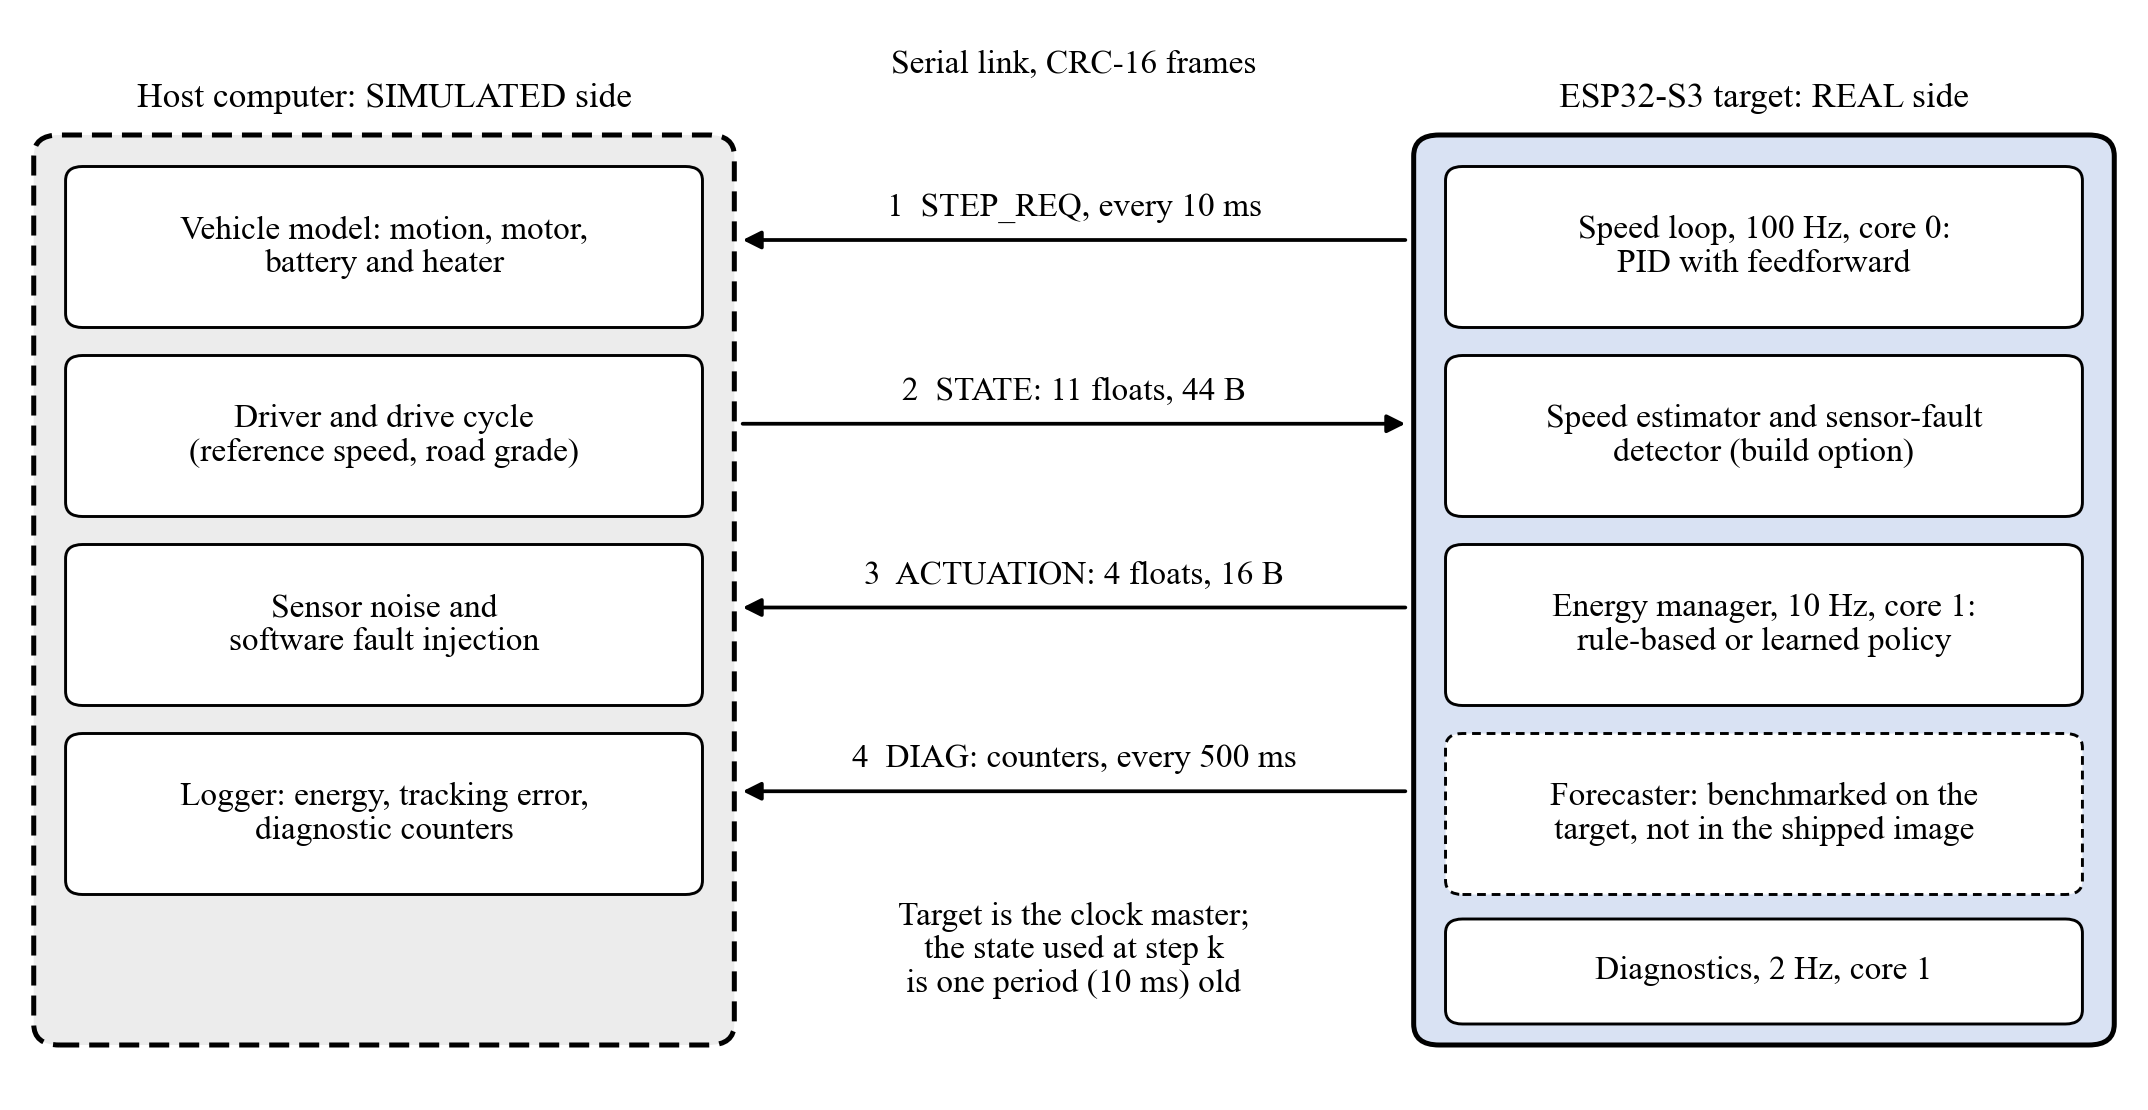
\includegraphics[width=\textwidth]{figures/fig-platform-architecture.png}
\caption{Processor-in-the-loop arrangement. The host side is simulated; the target side is real. The forecaster was benchmarked on the target but is not part of the shipped image.}
\label{fig:platform-architecture}
\end{figure*}

\subsection{Target Hardware and Firmware}

The target has two Xtensa LX7 cores at 240 MHz and 8 MB of PSRAM, and its FreeRTOS firmware runs four tasks. The 100 Hz speed loop has core 0 and the highest priority; it is a different task from the energy manager. It combines a PID controller with a physics feedforward and, in some builds, a speed estimator and fault detector. Core 1 hosts the energy manager and an inference task at 10 Hz and a diagnostic task at 2 Hz, so inference cannot delay control.

Which energy manager runs is a compile-time choice: the firmware builds the learned policy when its generated weight header exists and the rule-based manager otherwise. A campaign therefore needs one image per controller, and a diagnostic counter of policy steps, which cannot be non-zero in the rule-based image, confirms the choice.

The firmware moved from the vendor framework to the Arduino core, which yields a different binary from the same source, so every gate was measured again: the forecaster took 35.03 ms instead of 36.46 ms and the policy 0.123 ms instead of 0.121 ms. The Arduino image carries radio stacks that nothing starts. The board's supply current was not measured in this study, so no result concerns the power drawn by the microcontroller itself.

\subsection{Real-Time Behaviour}

Gate G3 was measured over 59,650 control loops, ten minutes, against the target's own clock. On the first Arduino-core run every loop landed within 25 \textmu{}s of its slot, the worst control computation took 61 \textmu{}s and no loop missed its deadline (Fig.~\ref{fig:platform-jitter}).

\begin{figure}[!t]
\centering
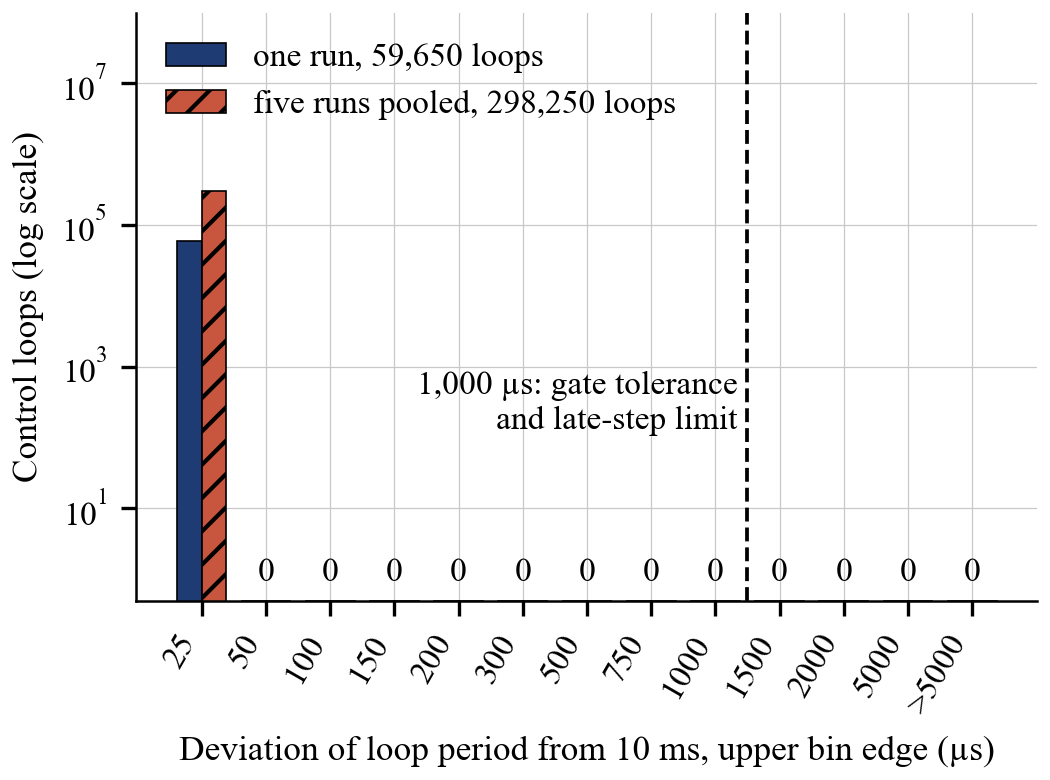
\includegraphics[width=\columnwidth]{figures/fig-platform-jitter.png}
\caption{Deviation of the control period from 10 ms on the Arduino-core build (target-measured). Empty bins are marked 0. The five pooled runs use the shipped image with the learned policy.}
\label{fig:platform-jitter}
\end{figure}

The frame criterion fails. A dropped frame is a reply that misses the 1 ms window. The first run had 9. All 121,208 frames arrived intact; the record attributes the misses to the host operating system answering late in bursts. Torque is ramped down only after more than five consecutive stale steps. That happened once.

Five repeats of the shipped image gave 16, 4, 6, 9 and 9 dropped frames, or 8.8 per run with a Poisson 95\% interval of 6.4 to 11.8; the events cluster, so the true interval is wider. Late control steps were 0 in every run, and the criterion was not loosened.

A stale state could bias the energy comparison of Section~\ref{sec:ems}. Across the 16 valid settings, the learned-minus-rules difference in dropped frames correlated with the energy difference at r = -0.03; no relation shows at this sample size, though a small effect is not excluded.

\subsection{Terms and Repetition}

An arm is a controller under test, and a setting (or cell) is one scenario level; the campaign sweeps six factors one at a time from a US06 baseline, at three levels each, for 36 runs across two arms. The two nonzero communication-delay settings, four runs, were excluded afterwards (Table~\ref{tab:platform-revisions}), leaving 32 runs in 16 valid settings. Five of the 16 are the same nominal US06 condition reached from different factors; the valid set holds 12 distinct conditions.

Energy is reported on the comparable scale: cabin heating that a controller sheds is added back at the energy it saved, and arms are ranked on the sum in Wh/km. Raw consumption would reward switching the heating off.

Seed 0, 1 or 2 is paired with the three levels of each factor and both arms receive the same draw, so within a factor the noise level is confounded with the seed, and the five nominal repeats hold at most three distinct draws. The plant and both controllers are deterministic, which means a repeat with the same seed replays the same noise draw and differs mainly in link timing, so it is not an independent repeat of anything the noise drives. The later fault campaign and the corrected-campaign repeats (Section~\ref{sec:ems}) add seed offsets of 100 and 200, giving three independent draws per condition.

Table~\ref{tab:platform-ledger} counts every energy-comparison run on the target and the reason any run left the analysed set; the run-level list, with source file and seed, is in the repository (Data and Code Availability).

\begin{table}[!t]
\centering
\caption{Ledger of energy-comparison runs on the target. Analysed runs include two offset-100 retakes that exceeded 16 dropped frames again and stand, as the rule allows one retake. The earlier campaigns predate the frame rule.}
\label{tab:platform-ledger}
\footnotesize
\setlength{\tabcolsep}{3pt}
\renewcommand{\arraystretch}{1.15}
\begin{tabularx}{\columnwidth}{@{}XXXXX@{}}
\hline
\textbf{Campaign} & \textbf{Attempted} & \textbf{Delay excluded} & \textbf{Set aside, frames} & \textbf{Analysed} \\
\hline
Earlier, faulty model & 36 & 4 & 0 & 32 \\
Earlier repeat, faulty model & 36 & 4 & 0 & 32 \\
Corrected, seed offset 0 & 40 & 4 & 4 & 32 \\
Corrected, seed offset 100 & 31 & 0 & 7 & 24 \\
Corrected, seed offset 200 & 29 & 0 & 5 & 24 \\
Speed-estimator blocks & 13 & 0 & 1 & 12 \\
\hline
\end{tabularx}
\end{table}

Anything written twice, in Python and in C, has a parity test; a policy network of the deployed shape matches its NumPy original to 2.12e-06. The host is kept idle during a campaign.

\subsection{Criteria Fixed in Advance, and What Was Decided Afterwards}

A criterion is written down before the experiment it governs. A result that misses it is reported as a miss. The five gate criteria were committed on 2026-08-30 with the design specification, before the commit that records the first gate measurement later that day. The criteria for the speed estimator and the first fault detector were committed on 2026-10-06, before any arm was run. Those for the bias-aware detector were committed on 2026-10-08 in the same commit as its code, so they preceded every learned reviewer but not the detector itself, whose step threshold was tuned on training data only. The 2026-10-14 measurement round was planned and committed before its runs.

Table~\ref{tab:platform-gates} holds every such criterion in the paper. Six are missed. They are G2, the zero-drop part of G3, the estimator's clean-tracking bound, the first detector's false-alarm limit, the bias-aware detector's simulated detection limit and its alarm rate on interpolated 100 Hz logged trips. At the logs' own 10 Hz rate the detector meets its count limit, with 196 alarms at standstill set apart as the plan fixed. The comparison of the two energy managers had no outcome criterion; its acceptance rule, dated 2026-09-21, required only that the 36 runs be recorded, and no later record adds one, so the comparison is descriptive (Section~\ref{sec:ems}). A ridge regression passed G4 before any proposed forecaster existed.

\begin{table*}[!t]
\centering
\caption{Every criterion fixed in advance in the paper, with the date of its record and its outcome.}
\label{tab:platform-gates}
\footnotesize
\setlength{\tabcolsep}{3pt}
\renewcommand{\arraystretch}{1.15}
\begin{tabularx}{\textwidth}{@{}XXXXX@{}}
\hline
\textbf{Id} & \textbf{Criterion fixed in advance} & \textbf{Fixed} & \textbf{Outcome} & \textbf{Label} \\
\hline
G1 & 0.1 M multiply-accumulates in 20 ms or less & 2026-08-30 & Pass: 3.30 ms from measured throughput, margin 6.1x & target-measured \\
G2 & Power RMSE within 10\% of mean; final SOC within 2 points & 2026-08-30 & Fail on 1 of 7 trips: SOC 2.45 against 2.00 & host-simulated \\
G3a & 99th-percentile period jitter of 1 ms or less & 2026-08-30 & Pass: 25 \textmu{}s & target-measured \\
G3b & Zero dropped frames in 10 min & 2026-08-30 & Fail: 4 to 16 per run & target-measured \\
G4 & 10\% lower RMSE than persistence at 3 s & 2026-08-30 & Pass: 14.5\% for the weakest fitted model & host-simulated \\
G5 & 40 ms or less; model plus arena 300 KB or less & 2026-08-30 & Timing and memory pass: 36.46 ms, 35.03 ms; 28,894 B. Converted model not yet run on target & target-measured \\
Ablations & Null result accepted in advance for physics loss and for forecast in the policy state & 2026-08-30 & Both null; forecast ablation on the corrected model +0.262 Wh/km, interval -0.698 to +0.982 & host-simulated \\
Headroom & Rule-based manager within 0.5\% of the DP reference on the corrected plant & 2026-10-14 & Met: 0.01\% to 0.16\%, unchanged by the fix & host-simulated \\
Bias-aware detector, logged trips, 10 Hz & Under 1 false alarm per clean hour on 70 trips (30.4 h), standstill alarms set apart & 2026-10-14 & Met numerically: 0.99 per hour on channels assumed healthy; flag up 59\% of recorded time & host-simulated \\
Bias-aware detector, logged trips, 100 Hz & Same limit, logged channels interpolated to 100 Hz & 2026-10-14 & Fail: 16.2 alarms per hour; interpolation, not a 100 Hz sensor & host-simulated \\
Plant sensitivity & Sign of learned minus rules unchanged in every plant variant & 2026-10-14 & Met: learned worse in all 14 variants, by 0.12\% to 0.81\% & host-simulated \\
Low-pass comparator & Credit filtering in general if the low-pass recovers at least as much 10x loss as the Kalman estimator & 2026-10-14 & Not met: less in both blocks, by 0.47 and 0.07 Wh/km, of the order of run spread & PIL-evaluated \\
Corrected comparison, three draws & Learned used more if exact two-sided Wilcoxon p \textless{} 0.05 with positive median over 12 conditions & 2026-10-14 & Met: higher in 12 of 12, median +0.50\%, p = 0.0005 & PIL-evaluated \\
Speed estimator & Clean energy within 0.2\% of the baseline loop & 2026-10-06 & Pass & PIL-evaluated \\
Speed estimator & Clean tracking within 0.005 m/s of the baseline loop & 2026-10-06 & Fail: 0.0193 against 0.0104 m/s on UDDS & PIL-evaluated \\
Speed estimator & At least half of the 10x-noise penalty recovered & 2026-10-06 & Pass: 9.44 to 0.24 Wh/km & PIL-evaluated \\
Speed estimator & Tracking below 0.1 m/s in every cell & 2026-10-06 & Pass & PIL-evaluated \\
First detector & No false alarm on a healthy sensor & 2026-10-06 & Fail: 1 false alarm on the target & PIL-evaluated \\
Bias-aware detector & Every named fault flagged within 0.5 s; under 1 false alarm per clean hour & 2026-10-08 & Not met: 551 and 533 of 560 caught & host-simulated \\
Bias-aware detector & Same limits on the target & 2026-10-08 & Met on cases run: 120 of 120 within 0.32 s; 0 alarms in 1 clean hour & PIL-evaluated \\
\hline
\end{tabularx}
\end{table*}

Table~\ref{tab:platform-revisions} records each rule or revision made after results were seen. The re-run rule and the delay exclusion are judgement calls. The origin of the 16-frame threshold is not recorded; it equals the largest count among the five G3 repeats, but the record does not say it came from them.

\begin{table*}[!t]
\centering
\caption{Rules and revisions made after results were seen.}
\label{tab:platform-revisions}
\footnotesize
\setlength{\tabcolsep}{3pt}
\renewcommand{\arraystretch}{1.15}
\begin{tabularx}{\textwidth}{@{}XXXX@{}}
\hline
\textbf{Change} & \textbf{Recorded} & \textbf{Prompt} & \textbf{Effect} \\
\hline
G2 split into three parts & 2026-08-30 & Pooled form failed all 7 trips & Both thresholds kept, a torque bound added; gate fails 1 of 7 \\
Delay settings excluded & 2026-09-21 & Neither arm followed the cycle (25.7 to 43.4 m/s) & Rule: tracking error 1 m/s or more; 4 of 36 runs dropped \\
Re-run above 16 dropped frames & 2026-10-07 & Four rule cells run beside other jobs (21 to 54) & Looser than G3; 17 energy-campaign and 8 fault-campaign runs set aside and retaken (Table~\ref{tab:platform-ledger}) \\
Deployed policy seed & 2026-10-06 & Five retrained seeds & Lowest HWFET validation energy, seed 3; US06 not used for the choice \\
Plant fix and added checks & 2026-10-06 & Anomalies in campaign tables, not a gate & 8.28\% gain withdrawn; limit-invariance sweep and reference check added \\
Second fault detector & 2026-10-08 & First detector assumed an acceleration channel that logged trips did not match & Offset state added; criteria recorded with it \\
Fused backup speed & 2026-10-09 & Checker with rule monitor failed on a heavier car & 18 candidates on one training cycle; rule fixed before runs \\
Frozen test disabled in log replay & 2026-10-14 & Standstill alarms dominated the 10 Hz count & Diagnostic outside the plan: 1.9 alarms per hour, flag up 21\%; not a criterion \\
Nominal row of the three-draw test & 2026-10-14 & Final plan review & Bookkeeping: the nominal condition is the aggressive-mixed cell, seeds 2, 102 and 202; the other four original nominal rows stay descriptive \\
\hline
\end{tabularx}
\end{table*}

\section{VEHICLE MODEL AND THE POWER-LIMIT ARTEFACT}
\label{sec:plant}

Every controller in this study acts on a simulated vehicle, so a fault in that vehicle enters every comparison. One such fault produced an 8.28\% mean energy saving for the learned policy that did not exist. This section describes the model, what its validation did not test, and the fault, its discovery and the checks it implies.

\subsection{Data}

The model was identified and validated on a public archive of 70 trips of a BMW i3~\cite{i3data}, logged every 0.1 s. Eligibility tests were fixed before any fit: state of charge (SOC) present, no charging, and two heater-power channels present and in agreement. Thirty-three trips passed, all in winter, so the validated envelope has a mean ambient temperature from -3.3 to 10.2 \textdegree{}C. The 33 were split by trip into 19 for identification, 7 for validation and 7 sealed for a final test that has not been opened.

The Vehicle Energy Dataset (VED)~\cite{ved} served for a transfer check. The campaigns use three dynamometer schedules~\cite{epacycles}: the Urban Dynamometer Driving Schedule (UDDS, 1369 s, 11.99 km), the Highway Fuel Economy Test (HWFET, 765 s, 16.51 km) and the aggressive US06 schedule (600 s, 12.89 km).

\subsection{Longitudinal Model}

The force balance \eqref{eq:plant-force} sets the acceleration, with mass $m$, rotational mass factor $e$, speed $v$, wheel force $F_{t}$, rolling and drag coefficients $c_{rr}$ and $c_{d}$, frontal area $A$, air density $\rho$ and grade $\theta$.

\begin{equation}
\label{eq:plant-force}
m(1+e)\dot{v} = F_{t} - m g c_{rr}\cos\theta - \tfrac{1}{2}\rho c_{d} A v^{2} - m g \sin\theta
\end{equation}

Torque $T$ becomes wheel force through the gear ratio, wheel radius and drivetrain efficiency. Electrical power uses motor speed $\omega$ and an efficiency $\eta$ from a map identified on training trips only.

\begin{equation}
\label{eq:plant-motor}
\begin{gathered}P_{e} = T\omega/\eta(T,\omega) \;\; (T\omega > 0) \\ P_{e} = T\omega\,\eta(T,\omega) \;\; (T\omega < 0)\end{gathered}
\end{equation}

The battery is a first-order equivalent circuit with terminal voltage $V_{t}$, open-circuit voltage $V_{oc}$ at SOC $s$, current $i$, resistance $R_{0}$ and an $R_{1}C_{1}$ branch; its open-circuit curve, branch values and current limits are assumptions.

\begin{equation}
\label{eq:plant-battery}
\begin{gathered}V_{t} = V_{oc}(s) - i R_{0} - v_{1} \\ \dot{s} = -\frac{i}{3600\,C_{b}} \\ \dot{v}_{1} = \frac{i}{C_{1}} - \frac{v_{1}}{R_{1}C_{1}}\end{gathered}
\end{equation}

The auxiliary load is 543 W at rest (measured) plus 127.3 W per degree below a 21 \textdegree{}C setpoint (fitted); the cooling slope is unidentified, because every eligible trip is colder than the setpoint. Regenerative braking returns a fraction of the braking power, limited by an assumed 50 kW ceiling and the pack's charge current. Table~\ref{tab:plant-params} lists the main parameters.

\begin{table}[!t]
\centering
\caption{Main parameters of the i3 model, with the origin of each value.}
\label{tab:plant-params}
\footnotesize
\setlength{\tabcolsep}{3pt}
\renewcommand{\arraystretch}{1.15}
\begin{tabularx}{\columnwidth}{@{}XXX@{}}
\hline
\textbf{Parameter} & \textbf{Value} & \textbf{Origin} \\
\hline
Mass $m$ & 1270 kg & published kerb mass plus driver \\
Frontal area $A$ & 2.38 m\textsuperscript{2} & from published drag area and an assumed drag coefficient \\
Wheel radius, gear ratio & 0.3498 m, 9.665 & from tyre size; published \\
Motor limits & 250 Nm, 125 kW & published \\
Drivetrain efficiency $\eta_{d}$ & 0.95 & assumed \\
Rolling coefficient $c_{rr}$ & 0.01947 & identified, training trips \\
Drag coefficient $c_{d}$ & 0.2202 & identified, training trips \\
Rotational factor $e$ & 0.1706 & identified, training trips \\
Resistance $R_{0}$ & 0.010 ohm & identified, at lower bound \\
Capacity $C_{b}$ & 61.7 Ah & Coulomb counting of logged data \\
\hline
\end{tabularx}
\end{table}

\subsection{Validation Against Logged Trips}

Gate G2 was written before the fit. It replays a held-out trip's logged speed and passes only if every validation trip meets the bounds. The original single criterion pooled three models and failed all seven trips without saying which was at fault, so it was split into three parts with both original thresholds kept. Part A: torque inverted from the speed profile within 50\% of the logged-torque standard deviation, the only new number. Part B: battery power, driven by logged torque, within 10\% of mean absolute power. Part C: terminal SOC within 2 percentage points (pp).

The gate fails on Part C. Parts A and B pass on 7 of 7 trips (worst case 48.6\% and 8.3\%), and Part C on 6 of 7, with a median of 0.19 pp. Trip B08 misses by 2.45 pp against 2.00 pp (Fig.~\ref{fig:plant-validation}); the bound was kept and the miss recorded.

\begin{figure}[!t]
\centering
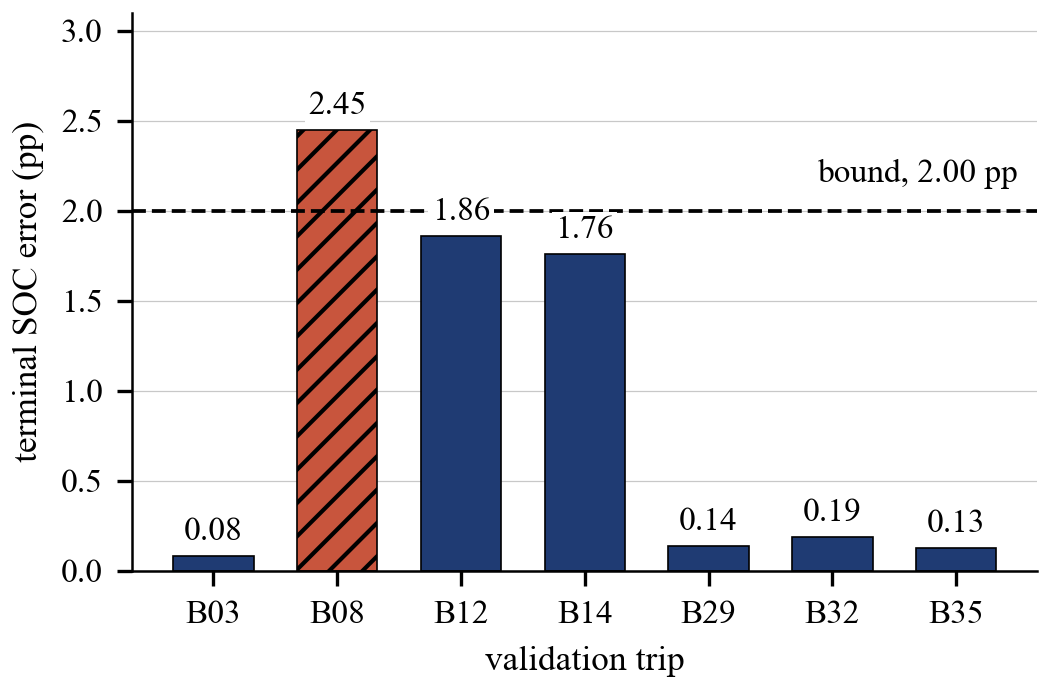
\includegraphics[width=\columnwidth]{figures/fig-plant-validation.png}
\caption{Terminal SOC error on the seven validation trips against the 2.00 pp bound of gate G2. Trip B08 (hatched) exceeds it. Host-simulated replay of logged trips.}
\label{fig:plant-validation}
\end{figure}

G2 checks the model along logged trajectories: logged torque goes in, and battery power and SOC come out. The controllers here send the model a battery power ceiling, and a replay of logged torque never asks the model to enforce one. The path that carried the fault below lay outside everything G2 exercised, so the gate could not have failed on it.

\subsection{Transfer to Another Vehicle}

The model was rebuilt around a 2013 Nissan Leaf from the battery-electric subset of VED and run on 89 validation trips. Arm A carried every i3 parameter across, arm B replaced the chassis coefficients with the Leaf's coastdown values, and arm C refitted the chassis. Median trip energy error was 16.9\%, 14.4\% and 13.4\% (host-simulated against logged trips).

\subsection{The Earlier Campaign and the Apparent Gain}
\label{sec:artefact}

The first processor-in-the-loop (PIL) campaign ran both energy managers on the ESP32-S3 target~\cite{esp32s3} against this model, over six factors at three levels each: 36 runs, 32 of them valid (Section~\ref{sec:ems}). The Soft Actor-Critic (SAC) policy~\cite{haarnoja2018} used less energy than the rule-based manager in 14 of 16 valid settings, by 8.28\% on average and by up to 21.6\% at driver aggression 1.5, on the comparable energy scale of Section~\ref{sec:platform} (PIL-evaluated). Fig.~\ref{fig:plant-reversal} shows each setting.

\begin{figure}[!t]
\centering
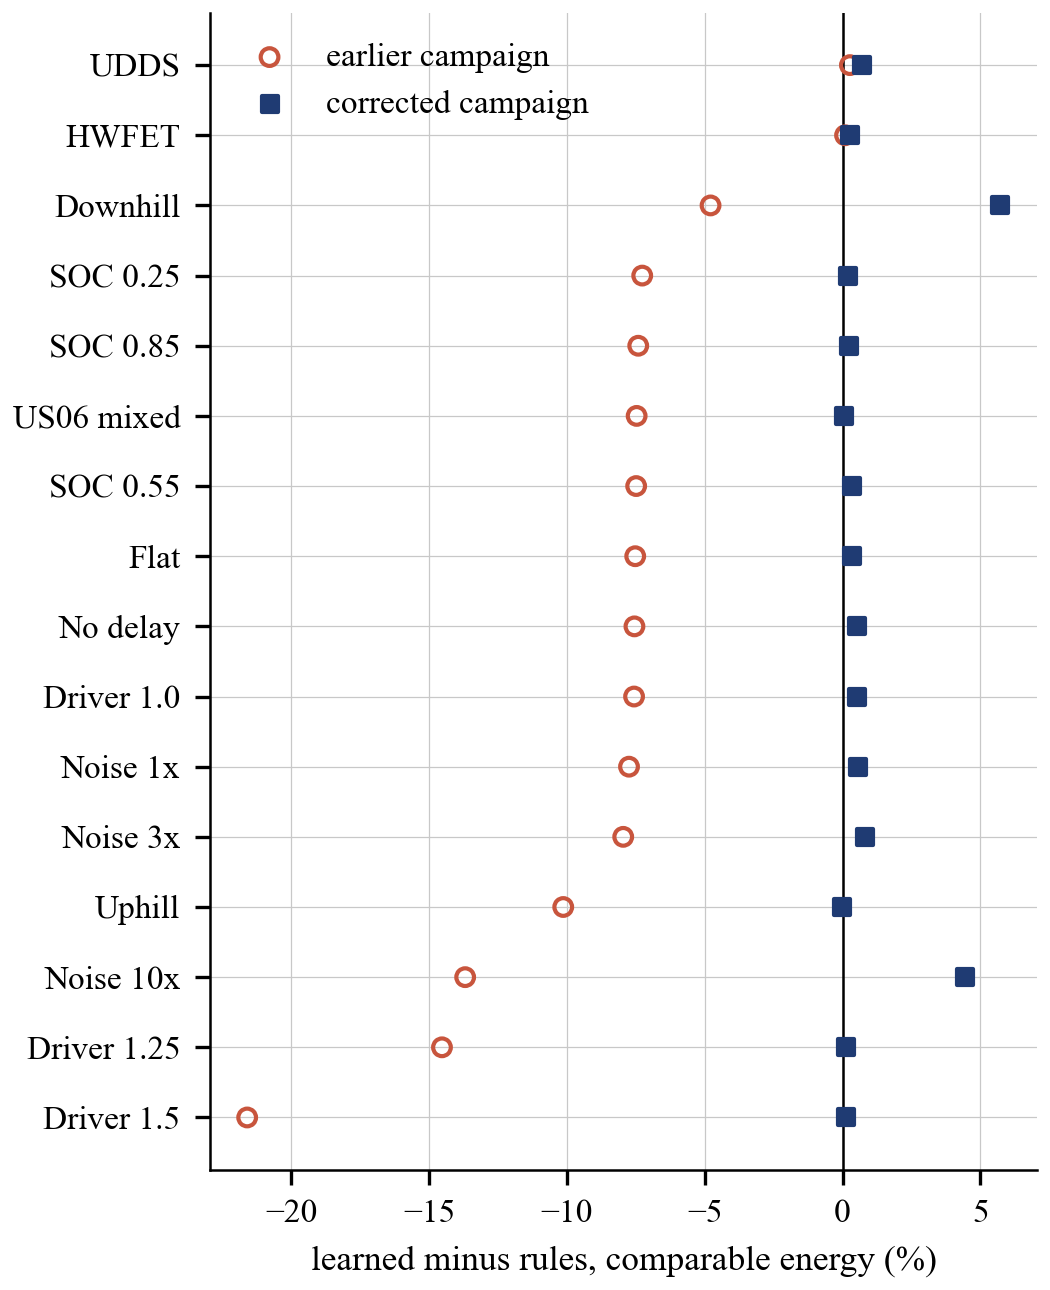
\includegraphics[width=\columnwidth]{figures/fig-plant-reversal.png}
\caption{Learned minus rule-based energy per setting on the comparable scale, in the earlier campaign on the faulty model and in the corrected campaign. Negative means the learned policy used less. PIL-evaluated, one run per cell; five of the 16 settings repeat the nominal US06 condition.}
\label{fig:plant-reversal}
\end{figure}

The gain rose with demand on three axes: 7.57\%, 14.54\% and 21.61\% across driver aggression 1.0, 1.25 and 1.5, and 4.79\%, 7.53\% and 10.14\% across downhill, flat and uphill. On the two gentlest cycles it was absent, with the learned policy using 0.27\% (UDDS) and 0.09\% (HWFET) more. A repeat campaign the next day, on firmware that also logged the discharge ceiling, reproduced it at 14 of 16 settings and 8.29\% (PIL-evaluated). The ceiling averaged 72.0 kW for the learned policy and 123.4 kW for the rules over the valid settings. A repeat shows that a result is reproducible on a model, not that the model bills fairly.

\subsection{The Mechanism}

Each energy manager sends the model a ceiling $P_{lim}$ on battery discharge power. The model applied it to the bill and not to the motion.

\begin{equation}
\label{eq:plant-limit}
P_{b} = \min(P_{m} + P_{a},\, P_{lim}), \qquad a = f(T_{req})
\end{equation}

Here $P_{m}$ is the machine power, $P_{a}$ the auxiliary load and $T_{req}$ the torque requested before any cap. The battery was charged $P_{b}$ while acceleration came from $T_{req}$, so billed and delivered power parted wherever demand exceeded the ceiling. A controller that lowered the ceiling was charged less and still received the motion it asked for.

The cause was isolated with no controller in the loop. A constant ceiling was held over US06 on the model before the fix, read from the repository history (Fig.~\ref{fig:plant-correction}, host-simulated). A 5 kW ceiling drove all 12.888 km at 8.05 Wh/km, with the same 0.0013 m/s tracking error as an open ceiling at 190.39 Wh/km. A constant 40 kW ceiling billed 174.85 Wh/km. The deployed learned policy, simulated on that model, scored 176.71 Wh/km against 176.53 measured on the target.

\begin{figure}[!t]
\centering
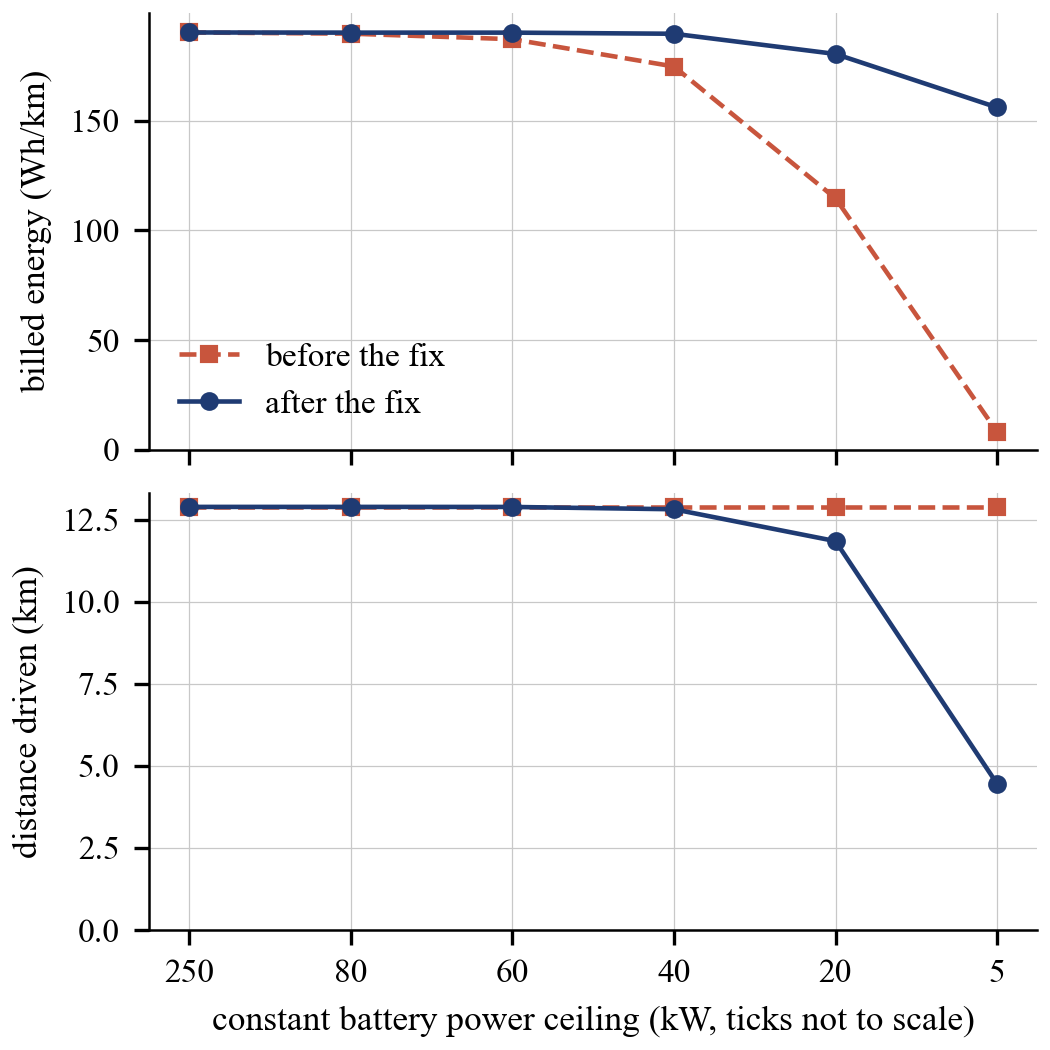
\includegraphics[width=\columnwidth]{figures/fig-plant-correction.png}
\caption{A constant battery power ceiling held over US06, before and after the fix, with no controller in the loop. Before, a lower ceiling cut the billed energy and left the distance unchanged; after, it also cuts the distance. Host-simulated.}
\label{fig:plant-correction}
\end{figure}

\subsection{How It Was Found}

The gates did not find it. G2 never exercised the ceiling path. The campaign tables carried three cues. The learned policy finished 7\% below the dynamic-programming (DP) reference of 190.39 Wh/km at equal tracking, a feasible policy the rules matched within 0.04\%; its advantage grew with demand; and it vanished on UDDS and HWFET, where demand stays under the 40 kW floor of the ceiling range. The fault was found 15 days after the first campaign.

The standing safeguards could not see it. G2 replays trips with a ceiling that never binds, the DP held the ceiling at the motor maximum by design, the plant's unit test asserted only that billed power met the ceiling, and the test that speed is unaffected by the energy action ran with a 300 kW ceiling. Two explanations recorded on the way, peak-current shaving and power limiting by the learned policy alone, were both wrong; the repeat campaign showed both controllers using the same 40 to 125 kW range but did not reveal the fault. The controller-free sweep did.

\subsection{The Fix and Its Consequences}

The fix gives the motor the power the pack delivered less the auxiliary load, reduces torque to match, and computes acceleration from the reduced torque. Four unit tests and one cycle-level test were added. Two limits that never bind give bit-identical outputs, and a starving ceiling must cost distance and tracking, not only the bill.

On the corrected model a 5 kW ceiling gives 156.16 Wh/km over 4.453 km with 16.15 m/s tracking error, and a 40 kW ceiling gives 189.80 Wh/km against 174.85 before (host-simulated). The rule-based manager and the DP reference did not change, since their ceiling never bound. The learned policy on US06 moved from 176.71 to 190.71 Wh/km, against 190.47 for the rules, with tracking error 0.48 m/s against 0.0013 m/s. On the target, across 16 valid settings, the corrected rule arm differed from the repeat campaign by +0.07\% on average (95\% interval -0.03 to +0.17\%), 0.46\% at worst, against 0.57\% at worst between two campaigns that differed only in the day (PIL-evaluated). The corrected comparison is in Section~\ref{sec:ems}.

\subsection{The Audit the Case Implies}
\label{sec:checks}

Fixing one billing rule is a repair. The reusable part is the audit, which asks whether every command a controller sends acts on the model's physics as well as on its energy account. Table~\ref{tab:plant-checks} sets it out in four groups, with the actuator path each check exercised, what it showed and what it leaves untested. All of these checks were written after the fault, and none was a gate fixed in advance.

\begin{table*}[!t]
\centering
\caption{Physical-consistency audit: what each check is for, the path it exercised, its result and its remaining coverage. Faulty means the pre-fix model loaded from the version history. Host-simulated.}
\label{tab:plant-checks}
\footnotesize
\setlength{\tabcolsep}{3pt}
\renewcommand{\arraystretch}{1.15}
\begin{tabularx}{\textwidth}{@{}XXXXXX@{}}
\hline
\textbf{Group} & \textbf{Check} & \textbf{Purpose} & \textbf{Path exercised} & \textbf{Observed} & \textbf{Coverage} \\
\hline
(i) Limits and conservation & Traction never exceeds what the battery supplied; a binding limit removes torque & Billed and delivered power must agree & Discharge-power ceiling; pack current limit & Faulty fails; corrected passes four unit tests and one cycle test & Tested \\
(i) Limits and conservation & Regeneration boundary against an oracle that does not call the plant helpers & Braking split, charge-current and SOC limits, terminal-port energy & Regeneration and charging & Seven cases pass on the corrected model & Tested, corrected model only \\
(ii) Controller-free sweep & Constant ceiling held over US06; energy and distance must fall together & A saving must carry a physical cost & Discharge-power ceiling, 5 to 250 kW & Faulty: 8.05 Wh/km at 5 kW, distance unchanged. Corrected: 156.16 Wh/km over 4.453 km & Tested \\
(ii) Controller-free sweep & Same sweep for the regeneration blend and the heater derate & As above & Blend; auxiliary derate & Only checked that the speed trace is unchanged & Recommended, not run \\
(iii) Non-binding invariance & A limit that does not bind leaves every output unchanged & A fix must not move unaffected arms & 250 kW against open ceiling; rule arm; DP reference & Bit-identical; rule arm +0.07\% on the target; all 28 stored results reproduced & Tested \\
(iv) Reference anomaly & A learned result well past a feasible reference on the same model opens an audit & Flag results the action space should not allow & All three actions together & Triggered: 176.71 against 190.39 Wh/km & Applied once, after the fact, in one direction \\
\hline
\end{tabularx}
\end{table*}

The anomaly trigger needs care. A learned result past a reference policy is a reason to investigate, not proof of a model defect: the learner may have found a larger action space, a weakness of the approximate reference, or a hole in the model. Here it was applied after the fact and only because the result favoured the learned policy; a fault that made the policy look worse would not have drawn the same scrutiny, and no symmetric audit was run. The pack current limit had the same fault as the power ceiling and was fixed in the same commit.

The plant tests that predate the fault already covered the five paths through which energy is billed: discharge-power and discharge-current limits, regenerative charge and SOC limits, auxiliary accounting, and energy integration. What they lacked was a check that a limit acts on motion. The faulty plant, run again from the version history, still gives 8.05 Wh/km at 5 kW, while the corrected plant reproduces its binding controls and leaves the 250 kW control and the rule arm unchanged (host-simulated).

\subsection{Limits of Plant Fidelity}

The three identified chassis coefficients do not measure what they are named after. The fitted rolling coefficient of 0.01947 is 2.2 times the 0.00878 of a published coastdown test of a 2013 Nissan Leaf~\cite{inl2013leaf}. That is unlikely to be tyre rolling resistance alone; the value probably absorbs drivetrain and brake drag, efficiency-map error and unmodelled load, and the same holds for $c_{d}$ and the rotational factor of 0.1706. The 50 kW regeneration ceiling and the 0.95 drivetrain efficiency are assumptions, and $R_{0}$ sits at its lower bound. Table~\ref{tab:plant-validity} collects what the validation supports and what it leaves open.

\begin{table}[!t]
\centering
\caption{Validity of the vehicle model and the consequence for reported figures. Host-simulated against logged trips unless stated.}
\label{tab:plant-validity}
\footnotesize
\setlength{\tabcolsep}{3pt}
\renewcommand{\arraystretch}{1.15}
\begin{tabularx}{\columnwidth}{@{}XXX@{}}
\hline
\textbf{Evidence} & \textbf{Result} & \textbf{Consequence} \\
\hline
G2 parts A and B, 7 i3 trips & Pass on 7 of 7 (worst 48.6\%, 8.3\%) & Torque and battery-power paths fit the logs \\
G2 part C, terminal SOC & 6 of 7; trip B08 2.45 against 2.00 pp & SOC drift over a trip can exceed the bound \\
Ambient envelope & Trip means -3.3 to 10.2 \textdegree{}C, winter only; campaigns at 12 \textdegree{}C & Campaigns sit just above the validated range; cooling load unidentified \\
Transfer, Nissan Leaf, 89 trips & Median trip-energy error 13.4\% to 16.9\% & Absolute Wh/km uncertain at that scale \\
Rolling coefficient & 2.2 times a published coastdown value & Lumped losses; rule arm on US06 falls from 190.47 to 150.09 Wh/km with the published value \\
One-at-a-time sensitivity, 14 variants & Learned higher in all 14, by 0.12\% to 0.81\% & Paired ranking held; interactions untested \\
Sealed test trips & 7 trips, not opened & No final test of the model \\
\hline
\end{tabularx}
\end{table}

These limits threaten absolute figures first: Wh/km values in this paper belong to this model, not to a car. Setting the rolling coefficient to the published 0.00878 lowers the rule arm's energy from 190.47 to 150.09 Wh/km on US06 and from 153.90 to 112.34 Wh/km on HWFET (host-simulated).

A one-at-a-time sweep tested the ranking, varying the vehicle model while both controllers kept the nominal one: the published rolling coefficient, a rotational factor of 0, the regeneration ceiling at 0.8 and 1.2 times its value, and drivetrain efficiency 3 points either side, on US06 and HWFET (host-simulated, no sensor noise, one policy seed). The learned policy used more energy in all 14 cases, by 0.12\% to 0.81\%, against 0.36\% and 0.20\% for the unchanged model. Raising the regeneration ceiling changed nothing, because it does not bind upward.

Interactions are untested; the drag coefficient, the battery resistance at its lower bound and the temperature dependence were left alone, and the sweep does not reach the winter-only envelope. The DP reference of Section~\ref{sec:ems} comes from the same model and inherits its limits.

\section{ENERGY MANAGEMENT AFTER THE CORRECTION}
\label{sec:ems}

This section compares a hand-written energy manager with a learned one on the corrected vehicle model of Section~\ref{sec:plant}. Both run on the microcontroller. The question is narrow. With the speed profile fixed by a tracking loop and only three actuation numbers to choose, did the evaluated learned policy use less energy than the rules on the corrected vehicle model? It did not.

\subsection{Control Structure and the Rule-Based Manager}

Two loops share the vehicle. An inner speed loop runs at 100 Hz on the microcontroller and turns the speed reference into motor torque. A slower supervisory energy manager runs at 10 Hz and sends three numbers: the fraction of braking energy routed to the machine (regeneration blend), a ceiling on battery discharge power, and the fraction of the auxiliary load, mainly cabin heating, to shed. The energy manager cannot change the speed reference, so no controller can save energy by driving slower.

The rule-based energy manager is a pure function of state of charge (SOC) and speed, with no memory. Regeneration is full below SOC 0.85, tapers linearly to zero at 0.94, and fades out below 2 m/s so that stops stay predictable. The discharge ceiling is 125 kW above SOC 0.20 and falls linearly to 40 kW at SOC 0.07. Auxiliary shedding stays at zero above SOC 0.15 and rises to a cap of 30\% as the pack empties. Two of these constants copy plant limits (0.94 is the battery's maximum SOC and 0.07 its minimum); the others were set by engineering judgement and not tuned against any test cycle. Table~\ref{tab:ems-hyper} lists them next to the learned policy's settings.

\subsection{Headroom Under a Fixed Speed Profile}

An approximate feasible-policy reference was computed by dynamic programming (DP)~\cite{bellman1957} on the WLTC class 3b cycle and the three dynamometer schedules UDDS, HWFET and US06~\cite{epacycles}, at a starting SOC of 0.80 and 12 degrees C. The DP carries SOC as its only state, takes the slow branch of the battery model from a nominal forward run, and holds the discharge ceiling at the motor maximum, so its value function is approximate; the reference figure comes from running the derived policy through the full vehicle model. It is a feasible policy, not a certified optimum of the physical plant. The rule-based manager differs from the energy of this reference policy by 0.01\% to 0.16\%: 153.90 against 153.89 Wh/km on the highway cycle (HWFET), 167.93 against 167.67 on the urban cycle (UDDS), 190.47 against 190.39 on the aggressive cycle (US06) and 175.99 against 175.94 on WLTC class 3b (host-simulated). The reference policy is a constant instruction: recover as much braking energy as the pack accepts. The DP was run again on the corrected model and the gaps did not change, because its ceiling never binds. Re-solving it on SOC grids of 81 to 321 points and action sets of 6 to 77 combinations left the reference energy unchanged to three decimals on all four cycles (host-simulated), since every grid gave the same constant instruction. That check covers the grid only. Under the specified model and objective, the gap does not certify the largest saving physically attainable: the single SOC state, the exogenous slow branch and the fixed ceiling remain approximations.

The small gap follows from the structure. Acceleration depends on torque and grade alone, so regeneration blend and shedding cannot alter the speed trajectory, and a ceiling can only remove power the speed loop needs, which the tracking constraint forbids. Shedding is priced at the energy it saves, which makes it neutral. Against this reference a learned policy had little visible room, and the experiment cannot tell a good learner from a poor one by energy alone. A gain needs a task with headroom, and Section~\ref{sec:planning} shows where one exists.

\subsection{The Learned Policy}

The learned policy is trained with Soft Actor-Critic (SAC)~\cite{haarnoja2018}. It observes eight scaled quantities: SOC, speed, acceleration, battery temperature, road grade, tracking error, and the mean and maximum of the next 3 s of reference-implied traction power. It outputs the same three numbers as the rules, mapped affinely from $[-1, 1]$ to the physical ranges. The reward is the negative sum of battery energy, shed auxiliary energy at the price it saves, a tracking-error term and penalties for excess current and low SOC; Table~\ref{tab:ems-hyper} gives the weights. The deployed actor is 8-64-64-3 with 4,931 parameters. Training used the WLTC3B and UDDS cycles with the HWFET cycle for validation, five seeds of 200,000 steps each.

Only one reward design and one hyperparameter set were run. There was no sweep. The tracking deficit reported below may reflect the tracking weight. This was not tested.

\begin{table*}[!t]
\centering
\caption{Settings of the learned policy and the rule-based manager. Library values are defaults of the Stable-Baselines3 SAC class; the others are set in the training script.}
\label{tab:ems-hyper}
\footnotesize
\setlength{\tabcolsep}{3pt}
\renewcommand{\arraystretch}{1.15}
\begin{tabularx}{\textwidth}{@{}XXX@{}}
\hline
\textbf{Item} & \textbf{Value} & \textbf{Origin} \\
\hline
Actor and critic hidden layers & 64, 64 & script; 4,931 actor parameters \\
Learning rate & 0.0003 & library default \\
Batch size, replay buffer & 256, 1,000,000 & library default \\
Discount, soft-update rate & 0.99, 0.005 & library default \\
Entropy coefficient & automatic & library default \\
Steps before learning starts & 1,000 & script \\
Training steps, seeds & 200,000, 5 & script \\
Episode length & 300 outer steps (30 s) & script default \\
Reward: energy, shed heat & 1.0 per Wh each & script \\
Reward: tracking & 5.0 per m\textsuperscript{2}/s\textsuperscript{2} & script \\
Reward: current, low SOC & 2.0 per A s over limit; 50 per unit SOC below floor plus 0.02 & script \\
Rule thresholds & see text & judgement; two equal plant limits \\
\hline
\end{tabularx}
\end{table*}

The comparable energy scale charges shed cabin heat back at exactly the energy it saved, so a policy that switches the heater off cannot look efficient. All ranking uses it.

After the model correction, five seeds per arm were retrained and scored on HWFET (host-simulated). The arm without forecast channels reaches 154.86 +- 0.51 Wh/km (seed standard deviation) against 153.90 for the rules, and the arm with them reaches 155.12 +- 0.82. The no-forecast seed with the lowest validation energy, seed 3 at 154.21 Wh/km, was exported to the target. It costs 0.121 ms per decision on average and 19.3 KB on the ESP32-S3~\cite{esp32s3}, and its outputs match the host implementation to 2e-06 against a tolerance of 2e-05 (target-measured, on another seed of the same network). Everything below concerns this one deployed seed. The worst policy computation in the campaign loop took 0.84 ms.

\subsection{Forecast Ablation}

The forecast ablation removes two observation channels, the mean and maximum of the next 3 s of reference-implied traction power, which are computed from the reference speed. It is not the Transformer forecaster of Section~\ref{sec:forecast}, which never ran inside the energy-management loop. Seeds are paired. On the original vehicle model the difference (with minus without) is +0.240 Wh/km with a 95\% bootstrap interval of -0.669 to +1.228; after retraining on the corrected model it is +0.262 with an interval of -0.698 to +0.982 (both host-simulated, five paired seeds). Both intervals contain zero. No equivalence margin was set, so the result is the absence of a detected effect and not proof of none. Under a fixed speed profile the best action does not depend on what happens next, which agrees with the DP result. The deployed policy was trained without them.

\subsection{Corrected Campaign on the Target}

The campaign closes the loop in the processor-in-the-loop (PIL) arrangement: the speed loop runs on the microcontroller at 100 Hz and the energy manager at 10 Hz, and the host simulates the vehicle, motor, inverter and battery. An arm is one controller under test; a setting is one combination of conditions. Six factors were each swept across three levels, one at a time from a US06 baseline at 12 degrees C: driving cycle (UDDS, HWFET, US06), road grade (+0.03, 0 and -0.03 rad), starting SOC (0.85, 0.55, 0.25), sensor noise (1x, 3x and 10x a stated floor), communication delay (none, 10 ms, 30 ms) and driver aggression (a time scaling of the reference by 1.0, 1.25 and 1.5). Each setting ran once per arm: 36 runs, 32 of them in the valid set, and 2,282,832 control steps, none late against the loop's own deadline (step timing target-measured; energy and tracking PIL-evaluated).

The two delay settings above zero are excluded because the host cannot answer within the delay and neither controller follows the cycle (tracking error 25.7 to 43.4 m/s); the exclusion rule, a tracking error of 1 m/s or more, was fixed after those runs were seen, and the largest valid error is 0.504 m/s. The remaining 16 settings are not 16 distinct conditions. Five of them, labelled R in Table~\ref{tab:ems-campaign}, are the same nominal US06 condition (mixed driving, no delay, flat road, 1x noise, driver 1.0), reached through different axes; the SOC 0.55 setting starts at a different charge and is not one. The valid set therefore holds 12 distinct conditions. Three of the five repeats used noise seed 0, so they differ mainly in link timing and run order, which is why their spread is a floor on run-to-run variation and not a full estimate of it. The repeats below give that estimate.

The rule arm used 190.73 to 191.41 Wh/km across the five repeats, a range of 0.36\%, and the learned arm 191.43 to 191.98, 0.29\%. The difference in dropped frames between the two arms is unrelated to the energy difference (r = -0.03 over the 16 settings).

Table~\ref{tab:ems-campaign} and Fig.~\ref{fig:ems-campaign} give the per-setting result. The learned policy uses less energy in 1 of the 16 settings, uphill at -0.02\%, which is 0.05 percentage points below the lowest nominal repeat and smaller in size than the 0.36\% spread of the rule arm. Averaged over the 16 settings it uses 0.94\% more, with a median of +0.35\%. Counting each distinct condition once in this single-draw campaign, with the five repeats merged into their mean, the learned policy is higher in 11 of 12 (median +0.31\%, exact Wilcoxon p = 0.001). Two settings carry the mean. These are downhill (+5.71\%) and 10x sensor noise (+4.45\%).

\begin{table*}[!t]
\centering
\caption{Corrected PIL campaign, 16 valid settings, one run per setting per controller, comparable energy scale. R marks the five repeats of the nominal US06 condition; Mixed is that condition reached through the driving-condition axis. PIL-evaluated.}
\label{tab:ems-campaign}
\footnotesize
\setlength{\tabcolsep}{3pt}
\renewcommand{\arraystretch}{1.15}
\begin{tabularx}{\textwidth}{@{}XXXXXXX@{}}
\hline
\textbf{Setting} & \textbf{Cycle} & \textbf{Rules (Wh/km)} & \textbf{Learned (Wh/km)} & \textbf{Difference (\%)} & \textbf{Rules RMSE (m/s)} & \textbf{Learned RMSE (m/s)} \\
\hline
Urban & UDDS & 168.13 & 169.30 & +0.70 & 0.013 & 0.016 \\
Highway & HWFET & 153.96 & 154.40 & +0.29 & 0.004 & 0.004 \\
Mixed (R) & US06 & 191.41 & 191.48 & +0.03 & 0.044 & 0.226 \\
No delay (R) & US06 & 190.73 & 191.76 & +0.54 & 0.014 & 0.230 \\
Uphill 0.03 rad & US06 & 305.26 & 305.21 & -0.02 & 0.039 & 0.237 \\
Flat (R) & US06 & 190.75 & 191.43 & +0.36 & 0.015 & 0.229 \\
Downhill 0.03 rad & US06 & 79.30 & 83.83 & +5.71 & 0.010 & 0.193 \\
SOC 0.85 & US06 & 190.93 & 191.37 & +0.23 & 0.026 & 0.233 \\
SOC 0.55 & US06 & 191.00 & 191.63 & +0.33 & 0.027 & 0.195 \\
SOC 0.25 & US06 & 190.80 & 191.20 & +0.21 & 0.021 & 0.168 \\
Noise 1x (R) & US06 & 190.75 & 191.81 & +0.55 & 0.021 & 0.230 \\
Noise 3x & US06 & 191.33 & 192.90 & +0.82 & 0.014 & 0.218 \\
Noise 10x & US06 & 201.55 & 210.53 & +4.45 & 0.055 & 0.192 \\
Driver 1.0 (R) & US06 & 190.99 & 191.98 & +0.52 & 0.028 & 0.228 \\
Driver 1.25 & US06 & 197.16 & 197.38 & +0.11 & 0.045 & 0.331 \\
Driver 1.5 & US06 & 204.46 & 204.75 & +0.14 & 0.098 & 0.504 \\
\hline
\end{tabularx}
\end{table*}

\begin{figure*}[!t]
\centering
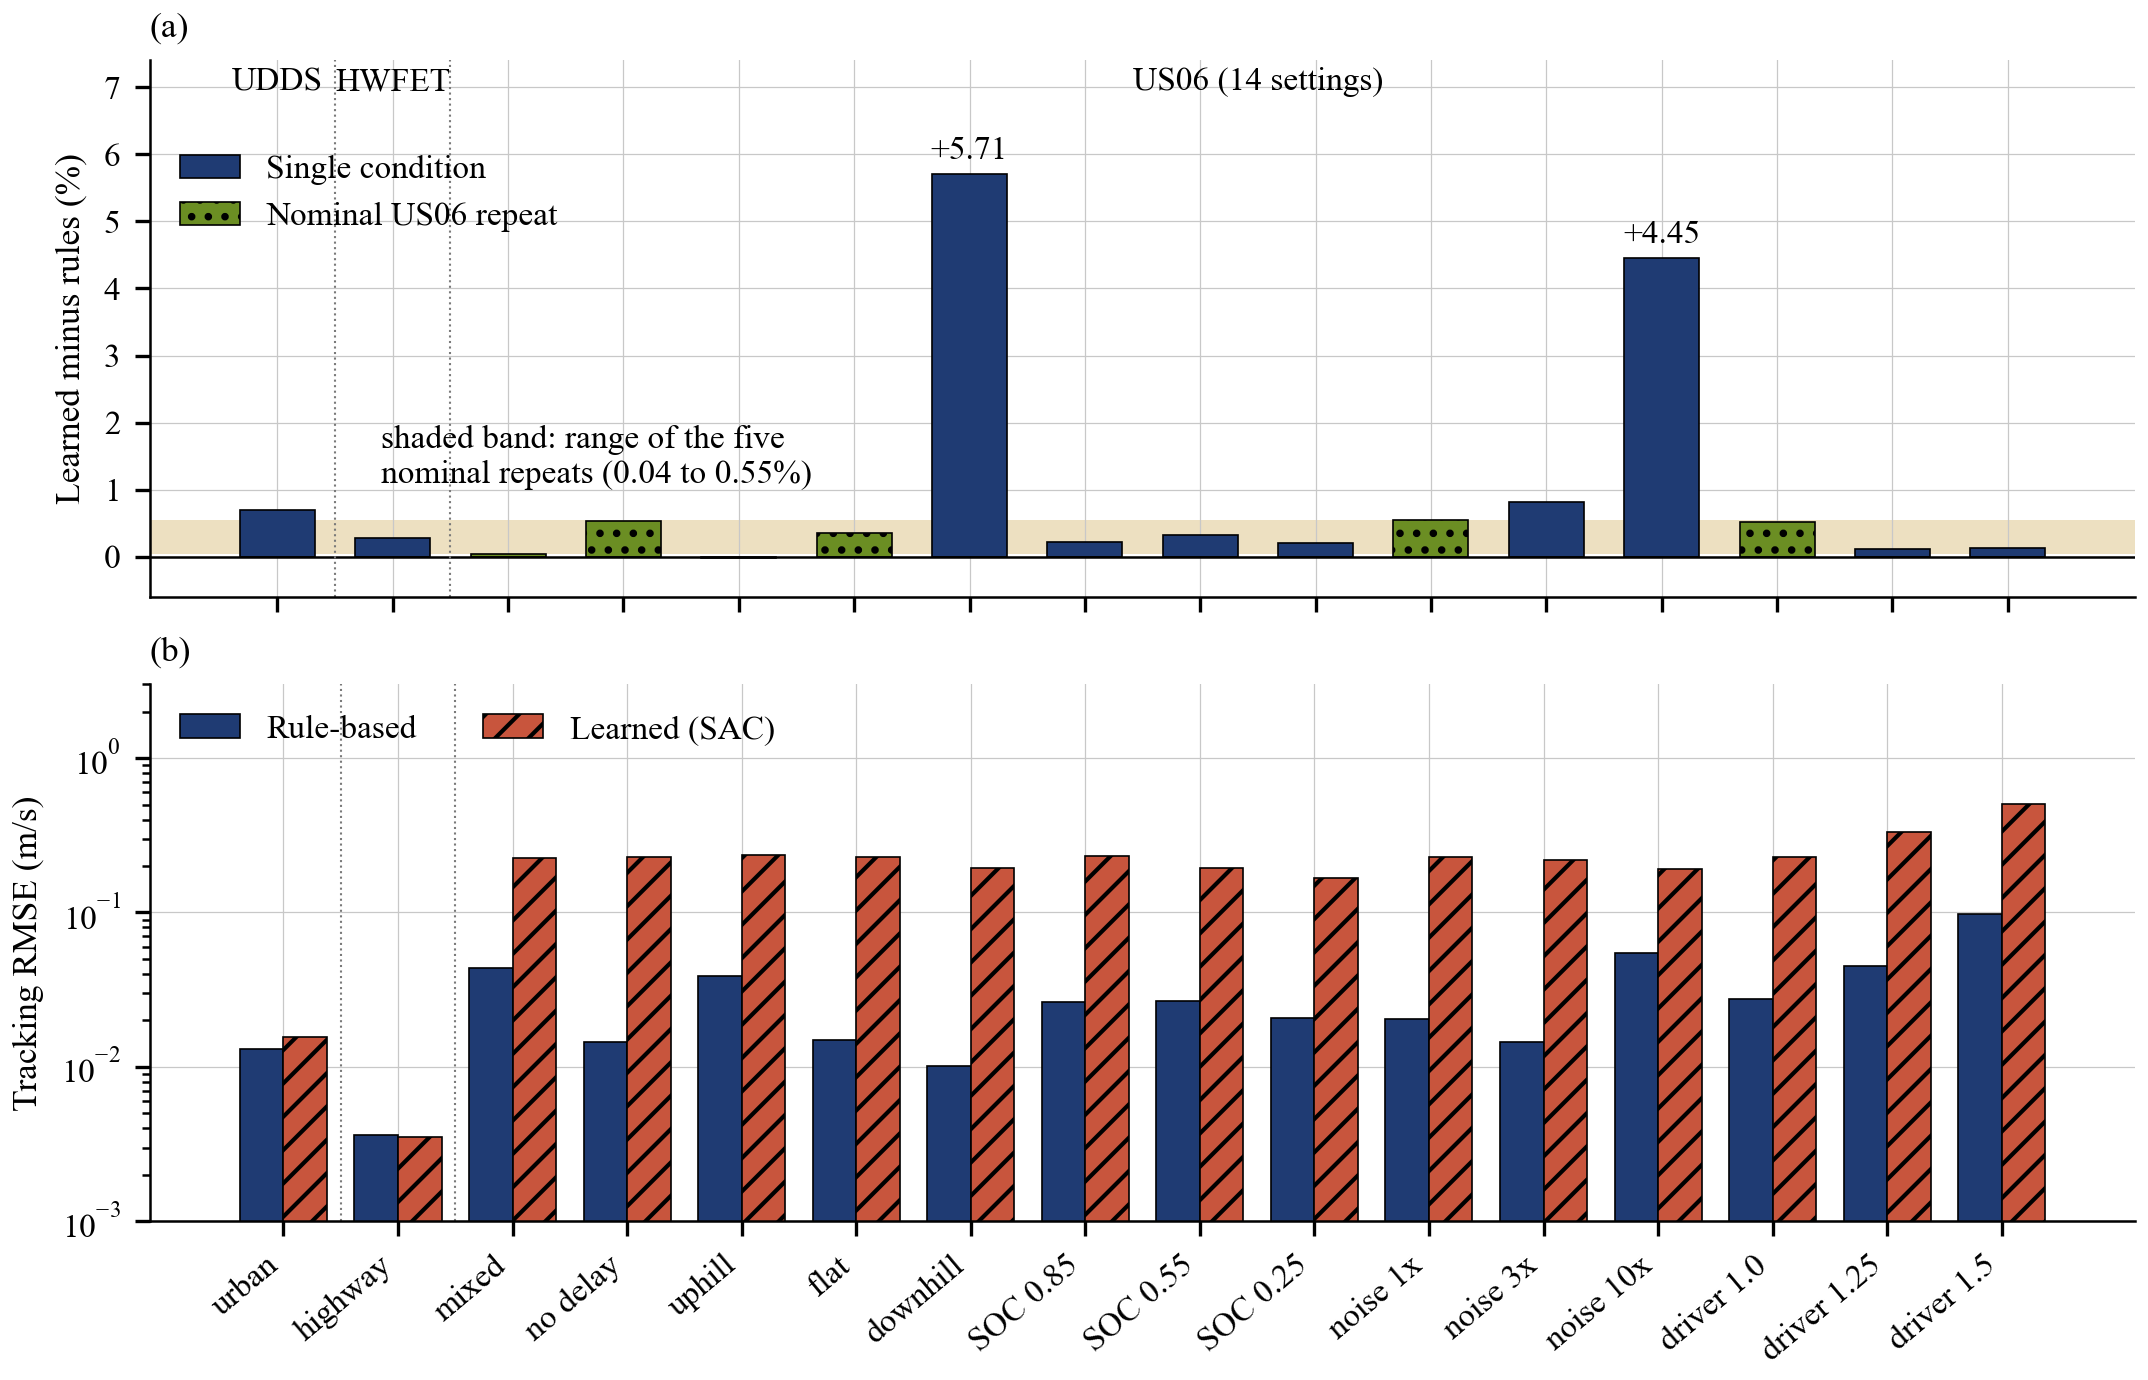
\includegraphics[width=\textwidth]{figures/fig-ems-campaign.png}
\caption{Corrected campaign, 16 valid settings: (a) paired energy difference of the learned policy relative to the rules, positive meaning more energy, with the range of the five nominal repeats as a shaded band and the repeats hatched; (b) tracking RMSE of both controllers on a log axis. PIL-evaluated, one run per setting.}
\label{fig:ems-campaign}
\end{figure*}

On tracking, the learned policy has a root-mean-square error (RMSE) of 0.17 to 0.24 m/s on most US06-based settings, 0.33 m/s at driver aggression 1.25 and 0.504 m/s at 1.5, against 0.010 to 0.098 m/s for the rules. On UDDS and HWFET the learned policy stays at 0.016 and 0.004 m/s.

The verdict covers this task only: one vehicle model at one ambient temperature, one board, one learned algorithm with one reward design, and speed fixed by the tracking loop. Varying the plant one parameter at a time left the sign unchanged (Section~\ref{sec:plant}). The result does not show that reinforcement learning cannot beat rules in general; it concerns one SAC implementation, one reward design and one deployed seed.

\subsection{Repeats With New Noise Draws}

Each of the 12 conditions then ran twice more per arm, with noise seeds offset by 100 and 200, the same build and re-run rule, and a test fixed before the runs (PIL-evaluated). The statistical unit is the condition. For each condition and draw the paired difference is 100(learned/rules - 1) on the comparable scale; the three draws are averaged, and the test runs over the 12 condition means. Same-seed runs of the first campaign do not enter as extra samples. The rule arm reproduced its first campaign within 0.57\% (median 0.15\%). Averaged over the three seeds, the learned policy used more energy in 12 of 12 conditions and in 35 of 36 paired runs, by a median of 0.50\% (bootstrap 95\% interval 0.30\% to 0.82\%). The exact two-sided Wilcoxon test over the 12 conditions gives p = 0.0005, meeting the criterion; the verdict stands (Table~\ref{tab:ems-repeats}). The learned arm also dropped more frames: 8 of its 24 new runs exceeded 16 and were retaken, against 4 for the rules; two retakes, at 23 and 55, stand under the rule. The run records, the analysis script and a ledger of every attempt are in the public repository, and one command regenerates the table and the test (Data and Code Availability).

\begin{table*}[!t]
\centering
\caption{Corrected campaign with three noise seeds per condition, comparable energy scale. Means of three seeds per arm; range is (max - min)/min of the learned arm; Nominal is the Mixed setting. PIL-evaluated.}
\label{tab:ems-repeats}
\footnotesize
\setlength{\tabcolsep}{3pt}
\renewcommand{\arraystretch}{1.15}
\begin{tabularx}{\textwidth}{@{}XXXXX@{}}
\hline
\textbf{Condition} & \textbf{Rules (Wh/km)} & \textbf{Learned (Wh/km)} & \textbf{Difference (\%)} & \textbf{Learned range (\%)} \\
\hline
Urban & 168.16 & 169.29 & +0.67 & 0.23 \\
Highway & 153.96 & 154.43 & +0.30 & 0.05 \\
Nominal & 191.02 & 191.58 & +0.29 & 0.14 \\
Uphill 0.03 rad & 305.05 & 305.31 & +0.09 & 0.09 \\
Downhill 0.03 rad & 79.45 & 84.55 & +6.42 & 1.65 \\
SOC 0.85 & 190.90 & 192.04 & +0.59 & 0.90 \\
SOC 0.55 & 191.02 & 191.82 & +0.42 & 0.50 \\
SOC 0.25 & 190.98 & 191.48 & +0.26 & 0.41 \\
Noise 3x & 191.68 & 193.55 & +0.97 & 0.80 \\
Noise 10x & 201.04 & 210.41 & +4.66 & 0.42 \\
Driver 1.25 & 196.96 & 197.79 & +0.42 & 0.54 \\
Driver 1.5 & 203.91 & 205.09 & +0.58 & 0.51 \\
\hline
\end{tabularx}
\end{table*}

\subsection{The Earlier Campaign}

An earlier campaign on the uncorrected model showed the opposite sign: the learned policy used less energy in 14 of the same 16 settings, by 8.28\% on average. That gain came from the vehicle model, not from the policy. Section~\ref{sec:plant} gives the mechanism, the controller-free sweep that exposed it and the checks it implies. After the fix and retraining it disappears.

\subsection{Behaviour Under Link Outage}

When the host link drops, the firmware reacts in two ways. If the 100 ms energy-manager setpoint is more than 300 ms old, the rule-based action runs inside the speed loop. If no vehicle state has arrived for more than five control periods (50 ms), the torque command is ramped to zero at 10 N m per step and the integrator is frozen. The fallback ablation compiles these two behaviours out; the firmware then holds the last command.

The sweep used outage lengths of 0.2, 0.5, 1, 2, 3, 4, 5 and 10 s, eight paired onsets on US06 per length, with the retrained policy in the loop and the corrected model (PIL-evaluated). Fig.~\ref{fig:ems-outage} shows the worst peak speed error. Removing the handling gives the smaller worst error from 0.2 s to 4 s (0.18 against 0.23 m/s at 0.2 s, 3.73 against 6.67 m/s at 4 s). At 5 s the order reverses, 7.40 m/s with the handling against 7.97 without, so the crossover lies between 4 and 5 s; no point inside that interval was measured. At 10 s the worst error is 13.3 m/s with the handling and 18.2 m/s without. The median is less regular: the handling has the lower median at 4 s (1.21 against 1.55 m/s) and at 10 s (3.72 against 5.33 m/s), and the higher one at 5 s (1.64 against 1.44 m/s).

\begin{figure}[!t]
\centering
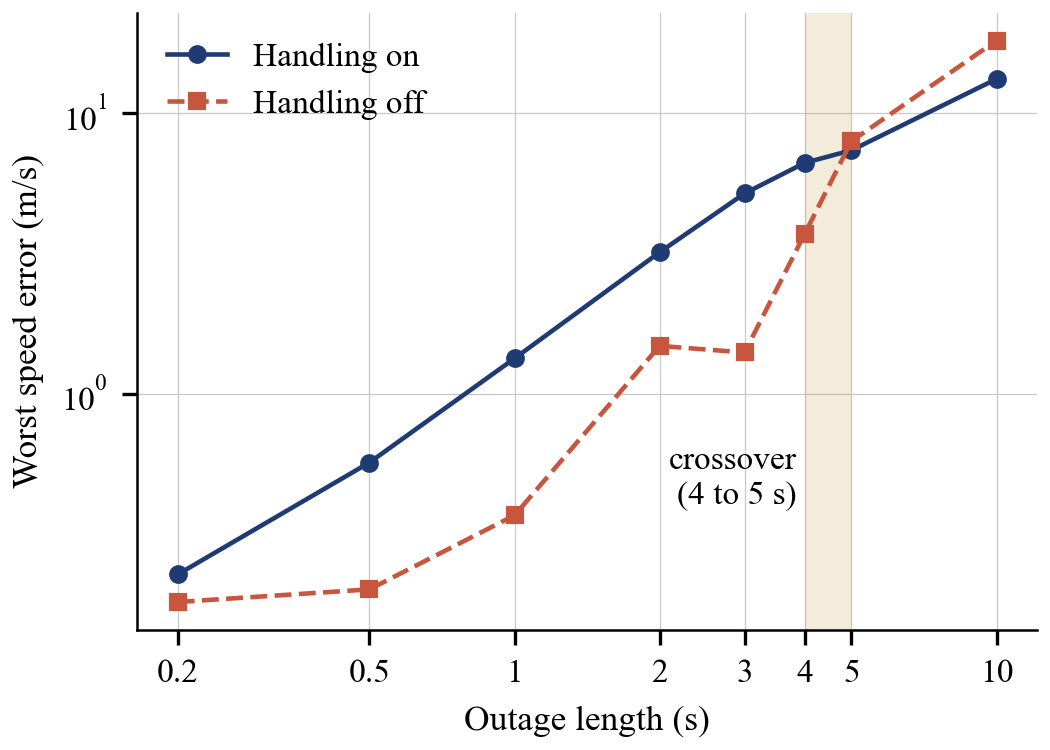
\includegraphics[width=\columnwidth]{figures/fig-ems-outage.png}
\caption{Worst peak speed error against outage length, with the fallback handling on and off, on the corrected model. PIL-evaluated, eight onsets per length; lines join measured points only.}
\label{fig:ems-outage}
\end{figure}

Holding a stale command works for a second or two and fails once the reference has moved on; the handling gives up accuracy early and loses less late. This is a description of behaviour under a link fault, not a functional-safety claim.

\section{ON-DEVICE FORECASTING: ACCURACY AGAINST COST}
\label{sec:forecast}

This section is a supporting result. A forecast of battery power for the next few seconds has to run on the same microcontroller as the control loop, so the question here is how accurate such a forecast can be and what each model costs on the ESP32-S3. The energy manager of Section~\ref{sec:ems} did not use any of these forecasters. Accuracy was computed on the host from validation trips (host-simulated); timings marked target-measured were taken on the target. The test trips were not opened.

\subsection{Task and Safeguards}

The task is to predict battery power at each of the next 30 samples, a horizon of 3.0 s at 10 Hz, from the preceding 32 samples (3.2 s) of eight signals: speed, acceleration, state of charge (SOC), battery current, battery voltage, ambient temperature, road grade and auxiliary power. Splits are by trip: 55,125 training windows from 19 trips and 29,252 validation windows from 7 trips.

Three safeguards were fixed before any model was fitted. Battery power is voltage times current and both are inputs, so inputs end at sample 32 and targets begin at sample 33, which an automated test asserts. A ridge regression with 257 parameters scored an $R^{2}$ of 0.4018 on real targets and $-0.0044$ on shuffled ones. Persistence holds the last value. It gives 13.219 kW of root-mean-square error (RMSE) at 3 s, and gate G4 requires 10\% below that, or 11.897 kW.

\subsection{Accuracy Against Cost}

The ladder runs, in order of cost, from persistence to linear regression, gradient-boosted trees (XGBoost)~\cite{chen2016}, a one-layer long short-term memory network (LSTM)~\cite{hochreiter1997} and a two-layer Transformer encoder~\cite{vaswani2017}. Table~\ref{tab:forecast-ladder} and Fig.~\ref{fig:forecast-cost} give the result. Each neural model is scored at its best validation epoch, so its error is slightly optimistic.

\begin{table*}[!t]
\centering
\caption{Forecast error at 3 s on validation trips (host-simulated) and cost on the ESP32-S3. Latency is target-measured where stated and otherwise estimated from operation counts.}
\label{tab:forecast-ladder}
\footnotesize
\setlength{\tabcolsep}{3pt}
\renewcommand{\arraystretch}{1.15}
\begin{tabularx}{\textwidth}{@{}XXXXXX@{}}
\hline
\textbf{Model} & \textbf{Error at 3 s (kW)} & \textbf{Gain over persistence (\%)} & \textbf{Size (KB)} & \textbf{Latency (ms)} & \textbf{Share of 40 ms budget (\%)} \\
\hline
Persistence & 13.219 & 0 & 0 & 0 & 0 \\
Linear regression & 11.308 & 14.5 & 7.5 & 0.26 (estimated) & 0.6 (estimated) \\
XGBoost & 11.290 & 14.6 & about 3,658 & not applicable & not applicable \\
LSTM & 11.120 & 15.9 & 20.4 & 35.07 (target-measured) & 88 \\
Transformer & 11.029 & 16.6 & 17.9 & 36.46 (target-measured) & 91 \\
\hline
\end{tabularx}
\end{table*}

Every fitted model passes G4, by at least 14.5\%. That settles little, because linear regression had already cleared the bar before the larger models existed, so the pass shows that a forecast is possible and says nothing in favour of a Transformer. Linear regression gives 87\% of the Transformer's gain for 1.2\% of its estimated compute. XGBoost is about twelve times over the 300 KB memory budget and stays as an offline reference. Seed spread within a model, 0.038 to 0.174 kW, is as large as the gaps between the top three.

\begin{figure}[!t]
\centering
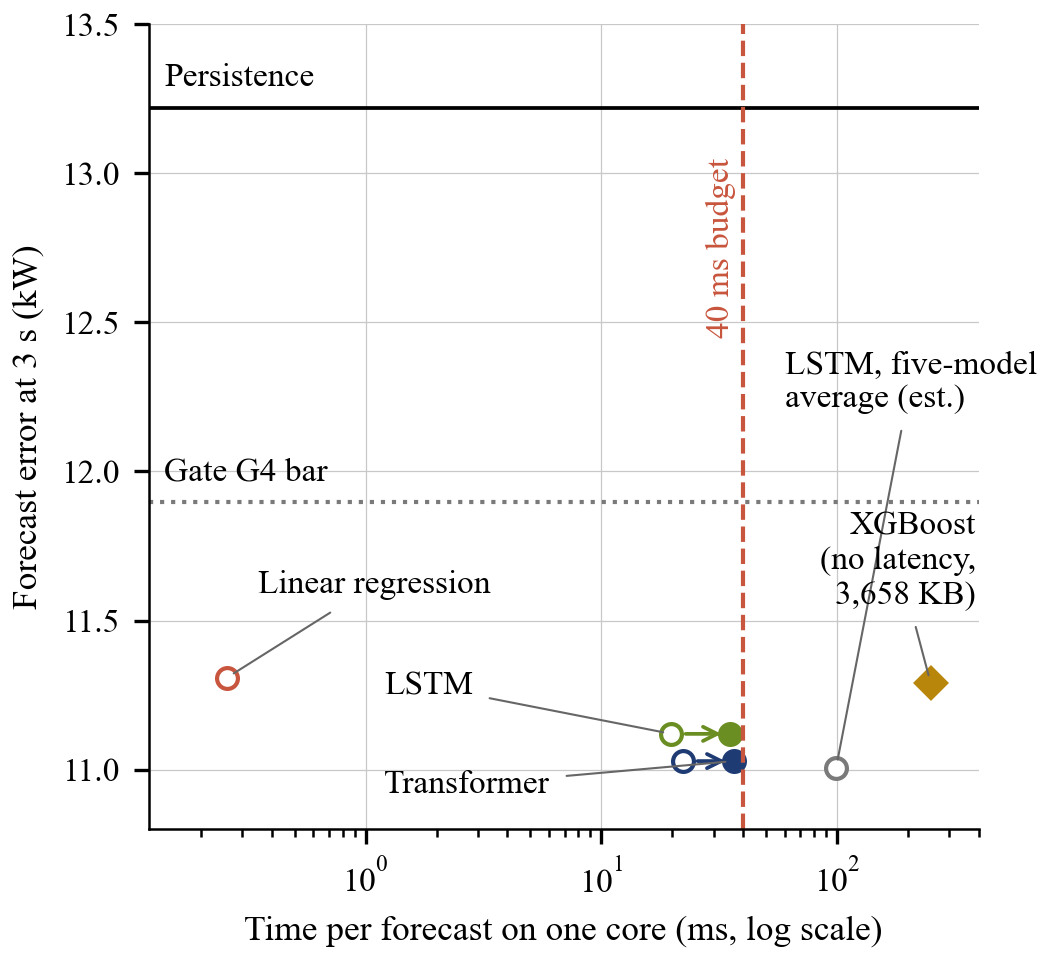
\includegraphics[width=\columnwidth]{figures/fig-forecast-cost.png}
\caption{Forecast error at 3 s against time per forecast. Open markers are estimates from operation counts; filled markers are target-measured on the ESP32-S3 (vendor-framework build). XGBoost has no latency figure and sits at the right edge.}
\label{fig:forecast-cost}
\end{figure}

\subsection{Cost on the Target}

The first Transformer cost, 22.28 ms, was the multiply-accumulate count divided by the throughput measured on the target. The same network in 8-bit C then took 36.46 ms per forward pass on the vendor-framework build, 91\% of the 40 ms budget of gate G5, and 35.03 ms on the Arduino core (target-measured). The measurement was 64\% above the estimate. Softmax, which needs 1,024 exponentials per head in each of four heads and two layers, and layer normalisation together account for 7.89 ms of the 14.18 ms gap, and the rest is not explained in the record. The LSTM has no softmax and was further off, 19.84 ms estimated against 35.07 ms measured, so the optimism lies in the method. Not the architecture. Operation counts can rank models. They should not set budgets. The timed code uses fixed weights, so it times the graph and says nothing about what a trained model would predict.

Rounding weights and activations to 8 bits~\cite{jacob2018} raised the error of the final-epoch model from 11.051 kW to 11.156 kW, a loss of 0.95\%, and shrank the stored model 3.6 times, from 71.7 KB to 20.2 KB (host-simulated). The timed graph needs 28,894 bytes, 9.4\% of the memory budget. Gate G5 is not closed in full. The converted model has not been run through an embedded runtime on the target, so the 8-bit accuracy is a host figure only.

Two further studies, both run on the host, added nothing to accuracy. A physics-informed loss~\cite{raissi2019} left the error unchanged, 11.057 kW against 11.052 kW, though it cut the share of steps where power disagrees with voltage times current by more than 500 W from 24.5\% to 2.5\%; consistency improved and accuracy did not. Distillation from a larger teacher~\cite{hinton2015} did not help. The students were worse by 0.20\% and 0.89\%, and the sign changed between seeds.

\section{SPEED ESTIMATION AND SENSOR-FAULT DETECTION}
\label{sec:estimation}

This section is a supporting result. The one energy gain found in the study sits in the speed loop, a level below the energy manager of Section~\ref{sec:ems}. Results are PIL-evaluated when the code ran on the ESP32-S3 in the processor-in-the-loop (PIL) arrangement, with computation times target-measured, and host-simulated when they ran on the host only. Faults were injected in software, and no physical accelerometer was used. The detector and fallback are evaluated as monitoring functions only; no ISO 26262 or safety-of-the-intended-functionality claim is made.

\subsection{Where the Noise Loss Sits}

Sensor noise raises the energy used under the rule-based manager. On US06 the energy, on the comparable scale of Section~\ref{sec:platform}, rose from 190.98 Wh/km at the noise floor to 200.42 Wh/km at ten times the floor (PIL-evaluated). The speed loop turns the reading into a torque command at 100 Hz, so noise becomes alternating drive and brake commands. Either the manager decides worse on a noisy state, or the loop wastes energy on the reversals.

Simulation supports the second reading: with the manager fixed, replacing only the speed estimate cut 200.3 to 190.6 Wh/km at ten times the noise and torque reversals from 1,342 to 83 per km (host-simulated, five seeds).

\subsection{Two-State Kalman Speed Estimator}

The estimator is a Kalman filter~\cite{kalman1960} over the speed $v$ and an unknown acceleration $d$, which absorbs what the vehicle model gets wrong, such as extra mass or headwind. The prediction advances the speed with the road-load model $a_{m}$ and the commanded torque $\tau$. On the target the state acted on is one request old, so the prediction uses the command before last; only the target exposed this.

\begin{equation}
\label{eq:estimation-predict}
\begin{gathered}\hat{v}^{-}_{k} = \hat{v}_{k-1} + \left[ a_{m}(\hat{v}_{k-1}, \tau_{k-j}) + \hat{d}_{k-1} \right] \Delta t \\ \hat{d}^{-}_{k} = \hat{d}_{k-1}\end{gathered}
\end{equation}

Here $j = 1$ in the host loop, $j = 2$ on the target, and $\Delta t$ is 10 ms. Process allowances of $q = 0.002$ m/s and $q_{d} = 0.02$ m/s\textsuperscript{2} were set on the first 600 s of the urban training cycle. The measurement $z_{k}$ corrects both states, with a variance $r^{2}$ re-estimated from the jitter of the reading.

\begin{equation}
\label{eq:estimation-update}
\begin{gathered}\nu_{k} = z_{k} - \hat{v}^{-}_{k} \\ S_{k} = P^{-}_{vv} + r^{2} \\ \hat{v}_{k} = \hat{v}^{-}_{k} + \frac{P^{-}_{vv}}{S_{k}} \nu_{k} \\ \hat{d}_{k} = \hat{d}^{-}_{k} + \frac{P^{-}_{vd}}{S_{k}} \nu_{k}\end{gathered}
\end{equation}

Two firmware images differing only in this input ran on the target, on three cycles at the noise floor, a second US06 noise seed, and US06 at three and ten times the floor. The baseline acts on the raw reading. Table~\ref{tab:estimation-noise} and Fig.~\ref{fig:estimation-noise} give the result.

\begin{table}[!t]
\centering
\caption{Energy on the comparable scale and peak battery current for the baseline loop and the two-state estimator, PIL-evaluated, one run per cell.}
\label{tab:estimation-noise}
\footnotesize
\setlength{\tabcolsep}{3pt}
\renewcommand{\arraystretch}{1.15}
\begin{tabularx}{\columnwidth}{@{}XXXX@{}}
\hline
\textbf{Setting} & \textbf{Baseline, Wh/km} & \textbf{Two-state, Wh/km} & \textbf{Peak current, baseline / two-state, A} \\
\hline
UDDS, floor & 168.10 & 168.05 & 118 / 111 \\
HWFET, floor & 153.98 & 153.92 & 97 / 92 \\
US06, floor & 190.79 & 190.61 & 284 / 262 \\
US06, floor, second seed & 190.98 & 190.56 & 295 / 260 \\
US06, 3x noise & 191.27 & 190.67 & 330 / 273 \\
US06, 10x noise & 200.42 & 190.80 & 341 / 288 \\
\hline
\end{tabularx}
\end{table}

\begin{figure}[!t]
\centering
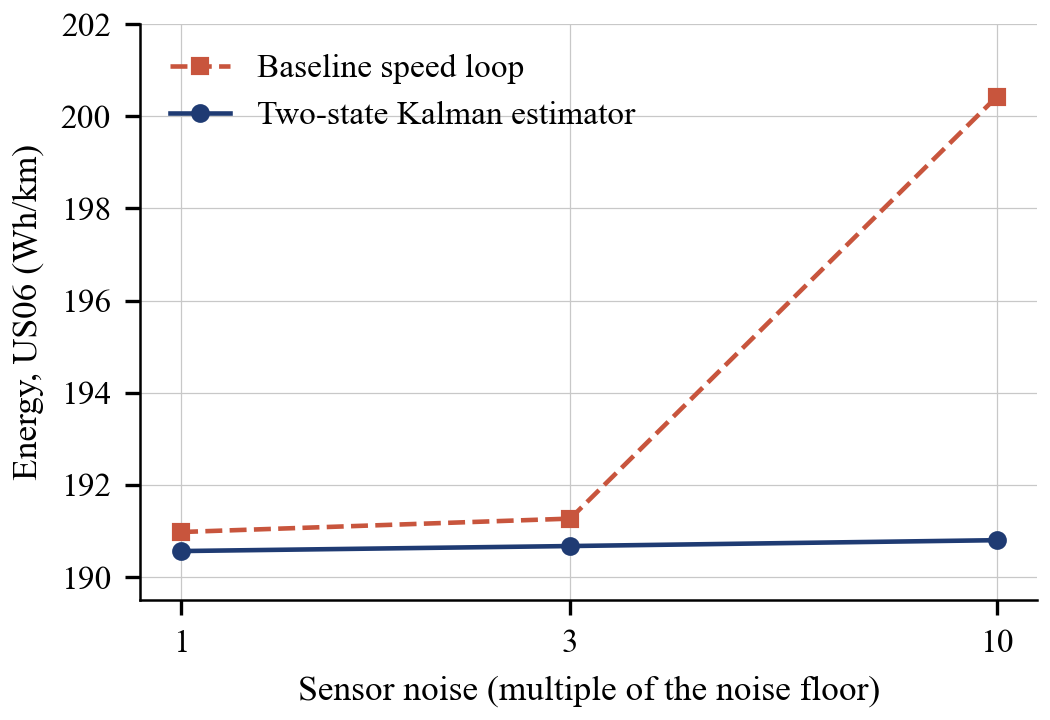
\includegraphics[width=\columnwidth]{figures/fig-estimation-noise.png}
\caption{Energy on US06 against sensor-noise multiple for the baseline speed loop and the two-state Kalman estimator, PIL-evaluated.}
\label{fig:estimation-noise}
\end{figure}

The headline loss is taken against the second US06 floor run. Against it the baseline loop loses 9.44 Wh/km (4.9\%) at ten times the noise and the two-state estimator 0.24 Wh/km; against the first floor run the losses are 9.63 and 0.19 Wh/km. The baseline's two floor runs differ by 0.19 Wh/km with only the noise seed changed, so the estimator's residual loss is about the size of run-to-run spread. The peak battery current falls from 341 A to 288 A, the worst control computation grows from 62 to 69 \textmu{}s of a 10,000 \textmu{}s period, and no step was late. At the noise floor the arms agree within 0.1\% on the three cycles and within 0.22\% on the second US06 seed, so no saving is claimed there.

The estimator was then set against a cheaper filter. A first-order low-pass filter on the reading, with its smoothing constant of 0.1 chosen on the training cycles at ten times the floor, ran beside the baseline and the estimator in two further noise blocks, at the floor and at ten times it (PIL-evaluated). Table~\ref{tab:estimation-lowpass} gives all three arms.

\begin{table}[!t]
\centering
\caption{Baseline loop, low-pass filter and two-state Kalman estimator on US06 in two noise blocks (floor seeds 100 and 200, ten-times seeds 102 and 202). Loss is ten-times energy minus the arm's own floor. PIL-evaluated, rule-based manager.}
\label{tab:estimation-lowpass}
\footnotesize
\setlength{\tabcolsep}{3pt}
\renewcommand{\arraystretch}{1.15}
\begin{tabularx}{\columnwidth}{@{}XXXXXX@{}}
\hline
\textbf{Arm} & \textbf{Block} & \textbf{Floor, Wh/km} & \textbf{10x, Wh/km} & \textbf{Loss, Wh/km} & \textbf{Floor RMSE, m/s} \\
\hline
Baseline & 100 & 191.15 & 200.80 & +9.65 & 0.035 \\
Baseline & 200 & 190.89 & 200.63 & +9.73 & 0.023 \\
Low-pass & 100 & 191.89 & 192.00 & +0.12 & 0.107 \\
Low-pass & 200 & 191.91 & 191.51 & -0.40 & 0.107 \\
Kalman & 100 & 191.14 & 190.78 & -0.36 & 0.035 \\
Kalman & 200 & 191.48 & 191.00 & -0.48 & 0.045 \\
\hline
\end{tabularx}
\end{table}

Most of the recovery belongs to filtering as such. Against the baseline of the same block the low-pass filter recovered 9.53 and 10.14 Wh/km and the estimator 10.01 and 10.21. The estimator's extra 0.47 and 0.07 Wh/km is of the order of run-to-run spread; the baseline's floor moved 0.26 Wh/km between blocks. The rule fixed beforehand would have credited filtering in general only if the low-pass filter recovered at least as much, so it is formally not met, but the margin does not justify crediting the energy recovery to the Kalman structure. The difference shows at the floor. The low-pass filter's clean energy was 0.38\% and 0.53\% above the baseline floor, and its clean tracking error was about three times higher, 0.107 against 0.023 to 0.045 m/s. What the estimator adds, on this evidence, is filtering without that clean-condition cost, on US06 and the seeds tested. Two blocks give a spread, not a population claim, and the estimator's floor tracking in them was four to five times its earlier run for a reason not established.

One criterion fixed before the run failed. Clean tracking on the urban cycle had to stay within 0.005 m/s of the baseline, and the estimator missed it by 0.004 m/s (0.0193 against 0.0104 m/s). The baseline's own two US06 floor runs differ by 0.011 m/s, so one run per cell cannot resolve the bound; it stays a failure because the bound was set first.

\subsection{Fault Detection From an Acceleration Residual, and Why It Failed}

The first detector compared the speed reading with a speed dead-reckoned from measured acceleration. With an idealised accelerometer it caught 160 of 160 named faults within 0.21 s and raised no false alarm in 3.8 h (host-simulated), but on the target it raised one false alarm on a healthy sensor in 1.26 h (PIL-evaluated). On the 70 logged trips, logged acceleration and the acceleration implied by logged speed differ by a slow component of about 0.11 m/s\textsuperscript{2}. Over the two-second pull of the dead reckoning that leaves a standing gap of about 0.22 m/s against a threshold of 0.036 m/s, and the detector was flagged 99\% of the time. It is not usable as tuned.

\subsection{Bias-Aware Fault Detector}

The bias-aware detector changes the reference the reading is tested against. The dead-reckoned speed carries a state $b$ for the acceleration-channel error, learned with a 2 s time constant and subtracted before integration. A step test handles abrupt faults: a sensor offset arrives in one sample and channel wander does not, so the mean gap $\bar{g}$ of the last $h = 30$ samples is compared with that of the 30 before.

\begin{equation}
\label{eq:estimation-step}
\left| \bar{g}_{\text{new}} - \bar{g}_{\text{old}} \right| > t_{s} \sqrt{\frac{2 \max(s^{2}, r^{2})}{h}} + \alpha h \Delta t
\end{equation}

Here $s^{2}$ is the pooled variance of the gap, $t_{s} = 6$, and $\alpha = 0.2$ m/s\textsuperscript{2} allows for a changing channel error. The threshold was tuned on the training cycles only; the cases and criteria were not altered after results were seen.

The simulated cases combine five named faults with six acceleration-channel errors, one of them the slow disagreement replayed from four logged trips per data split, and a vehicle 10\% heavier than the model. The detector raised no clean false alarm in 4.5 h on validation (HWFET) or 5.8 h on test (US06) and caught 551 and 533 of 560 named faults within 0.5 s (host-simulated), which misses the criteria fixed for it.

The detector was then replayed, settings unchanged, on the 70 logged trips at their native 10 Hz, 30.4 h in all (host-simulated replay). The trips carry no speed truth or health labels, so an alarm is false only if the channels were healthy, and the replay supplies zero torque and grade. Two quantities must be kept apart. Alarm onsets numbered 30, or 0.99 per hour, with 196 at standstill set apart under a rule fixed in advance; that meets the registered limit numerically but does not establish a population rate. The flag, however, was raised for a trip-weighted 59\% of recorded time, which no deployed detector could accept. With the frozen-speed test disabled, a diagnostic added after the result, onsets rose to 1.9 per hour. Interpolating the logged channels to 100 Hz and adding the noise floor gave 16.2 onsets per hour, almost all from the step test. Interpolation does not create a 100 Hz accelerometer, so that figure is a stress diagnostic, not a validation at the target rate. The detector is not field-ready, and the 120 of 120 below rests on software-injected faults on a simulated acceleration channel.

On the target the host injected the faults and simulated the accelerometer, and the detector ran in C, matched to the Python version on 4,000 samples. Table~\ref{tab:estimation-faults} and Fig.~\ref{fig:estimation-faults} give the result for US06 (PIL-evaluated).

\begin{table*}[!t]
\centering
\caption{Injected faults caught within 0.5 s on the target by fault type (PIL-evaluated). First campaign: 8 runs per type. Three noise draws: 24 runs per type.}
\label{tab:estimation-faults}
\footnotesize
\setlength{\tabcolsep}{3pt}
\renewcommand{\arraystretch}{1.15}
\begin{tabularx}{\textwidth}{@{}XXXXX@{}}
\hline
\textbf{Fault} & \textbf{Earlier detector, first campaign} & \textbf{Bias-aware, first campaign} & \textbf{Bias-aware, three draws} & \textbf{Worst tracking error, three draws, m/s} \\
\hline
Stuck & 7 of 8 & 8 of 8 & 24 of 24 & 0.62 \\
Dropout & 7 of 8 & 8 of 8 & 24 of 24 & 0.65 \\
Offset +0.5 m/s & 6 of 8 & 8 of 8 & 24 of 24 & 0.83 \\
Offset -0.5 m/s & 6 of 8 & 8 of 8 & 24 of 24 & 0.72 \\
Offset +3.0 m/s & 7 of 8 & 8 of 8 & 24 of 24 & 0.66 \\
All & 33 of 40 & 40 of 40 & 120 of 120 & 0.83 \\
\hline
\end{tabularx}
\end{table*}

\begin{figure}[!t]
\centering
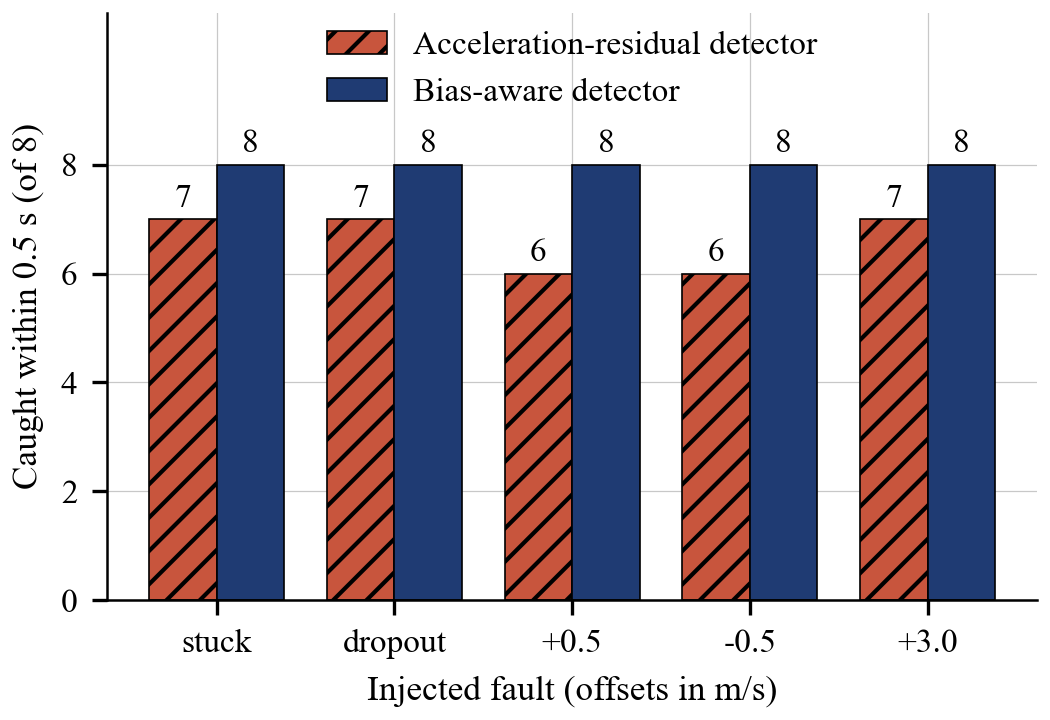
\includegraphics[width=\columnwidth]{figures/fig-estimation-faults.png}
\caption{Faults caught within 0.5 s in the first campaign on the target, earlier detector against bias-aware detector (PIL-evaluated). Eight faults per type.}
\label{fig:estimation-faults}
\end{figure}

In the first campaign the bias-aware detector caught 40 of 40 faults within 0.32 s; the earlier detector caught 33 of 40 and raised 162 false alarms on one clean cycle. The 120 of 120 is these 40 faults repeated over three noise draws, so it counts software faults on a simulated sensor, not independent events. The flag dropped while the fault persisted in 47 of the 120 runs. No false alarm occurred in the one clean hour, which bounds the false-alarm rate below about 3 per hour at 95\% confidence. No step was late; the worst control computation was 74 \textmu{}s (target-measured).

\subsection{Learned Reviewers Against a Rule Monitor}

A slower supervisory slot sits around the detector. Every 100 ms it receives twelve summary numbers and may hold or release a flag, switch the fallback speed or tighten the tests; it never commands torque. A hand-written rule monitor, a gated recurrent unit (GRU)~\cite{cho2014} of 1,508 parameters and a FastGRNN~\cite{kusupati2018} of 550 each filled the slot (host-simulated; the learned reviewers were not timed on the target). The GRU diagnosed better: while the detector's flag was down, it still labelled a real fault correctly in 88\% of blocks against 1\% for the monitor. In the loop the order reversed (Fig.~\ref{fig:estimation-reviewers}). The monitor cut the worst peak tracking error through a fault from 3.7 to 1.2 m/s on validation and from 5.1 to 1.4 m/s on test, while the GRU reached 9.7 and 10.8 m/s and the FastGRNN 3.0 and 12.8 m/s, and both raised clean false alarms.

\begin{figure}[!t]
\centering
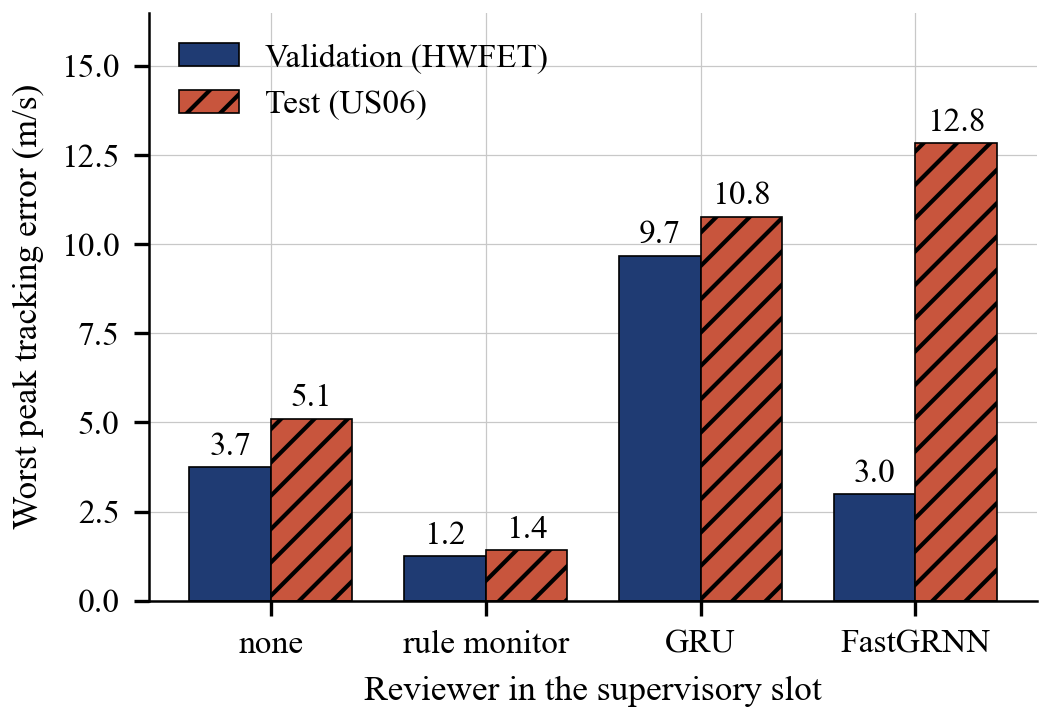
\includegraphics[width=\columnwidth]{figures/fig-estimation-reviewers.png}
\caption{Worst peak tracking error through any of 560 named faults for each reviewer on the controller with no delay (host-simulated). No reviewer means the bias-aware detector alone.}
\label{fig:estimation-reviewers}
\end{figure}

On the target the monitor looked slightly better than the detector alone in the first run (largest error 0.61 against 0.67 m/s) but worse over three noise draws, 1.32 against 0.83 m/s, with three alarms left raised (PIL-evaluated). No benefit is claimed.

\subsection{Fused Fallback Estimator}

A fused fallback estimator learns both fallback errors, from the acceleration channel and from the model, while the sensor is trusted and carries them through a flagged period. On the validation highway cycle its worst error was 0.62 m/s against 3.74 m/s for the detector alone; on US06 it was best in six of seven conditions and worst, at 2.59 m/s, with the vehicle 10\% heavier than the model, for a reason not tested. It has not been ported to C or run on the target (host-simulated only).

\section{SPEED PLANNING}
\label{sec:planning}

This section is a supporting result, and everything in it is host-simulated; nothing ran on the target. The energy managers of Section~\ref{sec:ems} could not change the speed trace, and that fixed trace is what left them almost nothing to win. Here the vehicle chooses the trace, so the headroom can be measured where it appears. Eco-driving is a long-standing optimal-control problem~\cite{sciarretta2015}.

A route is built from a standard drive cycle with the driver removed. It keeps the cycle's distance, its stops and the wait at each, a speed limit at every point, the hardest acceleration and braking the cycle used, and its duration as the arrival time within 1\%. The US06 and HWFET routes serve as test and validation sets.

Five arms were compared. The cycle as driven is the reference. A dynamic-programming (DP) planner~\cite{bellman1957} searches the whole route in 10 m steps, with a price on time set by bisection so that the planned arrival time is met. It solves the planner's own energy model, so it is a planning reference, not a certified optimum of the vehicle. The same planner was run with a 300 m horizon, replanning every 40 m, and again with a small network supplying a terminal cost, an estimate of what the rest of the route costs. The fifth arm is a student policy, a network trained on the planner's solutions that names the next speed directly. The learned arms see more than the 300 m arm: speed limits up to 700 m ahead, a stop cue up to 1300 m, and a feasibility mask computed over the whole remaining route, so the 300 m arm is not an equal-preview control. Every profile was driven through the full vehicle model with the speed loop and the rule-based energy manager, and energy is stated on the comparable scale (Table~\ref{tab:planning-savings}).

\begin{table}[!t]
\centering
\caption{Energy saved against the cycle as driven, by planning arm; one run per route, host-simulated, no other traffic.}
\label{tab:planning-savings}
\footnotesize
\setlength{\tabcolsep}{3pt}
\renewcommand{\arraystretch}{1.15}
\begin{tabularx}{\columnwidth}{@{}XXX@{}}
\hline
\textbf{Arm} & \textbf{US06 route (\%)} & \textbf{HWFET route (\%)} \\
\hline
Cycle as driven & 0.0 & 0.0 \\
DP, whole route & 10.4 & 1.2 \\
DP, 300 m horizon & 9.5 & 0.8 \\
300 m, learned terminal cost & 10.4 & 1.1 \\
Student policy & 0.03 & 0.3 \\
\hline
\end{tabularx}
\end{table}

On the US06 route the whole-route planner saved 10.4\% at the same stops and within the 1\% arrival tolerance. The HWFET route offered 1.2\%, since that drive has little to smooth. The terminal-cost arm matched the whole-route saving, but it planned to arrive 3.9 s later than the whole-route planner and 6.3 s later than the 300 m arm, with more preview than the latter, so no learned benefit is isolated. The student policy saved 0.03\% on US06. Arrival here is the planned time of the node profile, not the time the driven trace crossed the route's end, and the constraint counts describe the planned profile; closed-loop limit and stop compliance were not evaluated. Replayed from the frozen code, all eight runs reproduced, and every driven trace crossed the route's end about 6.2 s (US06) or 2.2 s (HWFET) before its planned time, so the gaps between arms hold (host-simulated).

An empty road is an optimistic scenario. As a surrogate for traffic constraints, the planner was held within a corridor around the recorded drive, ahead or behind, at every second, with distance and arrival time unchanged. Fig.~\ref{fig:planning-corridor} shows that the US06 saving was 5.1\% within 25 m and 9.7\% within 100 m, while HWFET stayed between -0.1\% and 1.7\%. The corridor planner differs in construction from the empty-road planner, so its 200 m figure of 12.6\% is not comparable with the 10.4\% above.

\begin{figure}[!t]
\centering
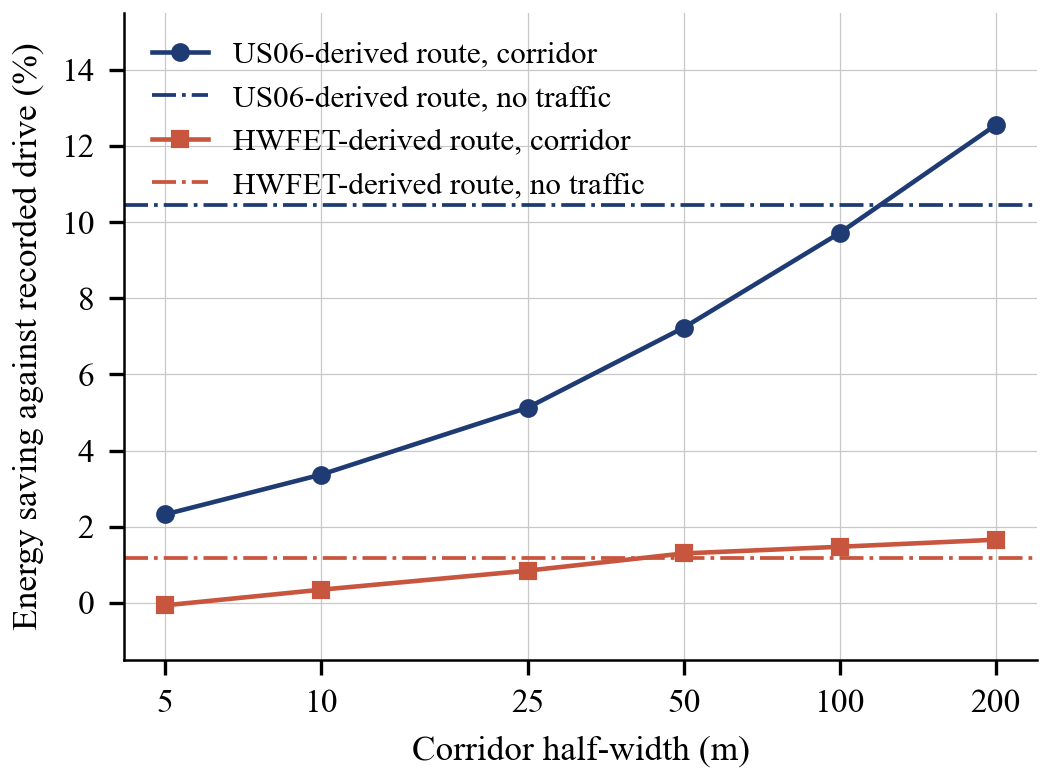
\includegraphics[width=\columnwidth]{figures/fig-planning-corridor.png}
\caption{Energy saving against corridor half-width, with the no-traffic saving as a dash-dotted reference line for each route. Host-simulated; one run per width.}
\label{fig:planning-corridor}
\end{figure}

Planning took 0.19 s in Python on the laptop for all 323 replans of the US06 route with the terminal cost; nothing was ported, so no time or memory on the target is claimed. The traffic is one recorded drive, with no other vehicle, hills or signals, and each arm was run once.

\section{DISCUSSION AND LIMITATIONS}
\label{sec:discussion}

\subsection{Why the Rules Held}

The comparison of Section~\ref{sec:ems} left little visible room for any controller. With the speed fixed by the tracking loop, three actuation numbers and cabin heat charged back at the energy it saves, a feasible policy derived by approximate dynamic programming and run through the full model differed from the rules by 0.01\% to 0.16\% on four cycles; refining its grid did not move it, and the fix did not either, because its discharge ceiling never binds. The gap is a difference from one evaluated reference policy and does not certify the largest saving physically attainable. Against it, with a tracking penalty to pay, the evaluated policy used more energy in 12 of 12 distinct conditions over three noise draws (host-simulated reference, PIL-evaluated campaign).

The null result is about this task. This SAC policy, with one reward design, one hyperparameter set and one deployed seed, found nothing on this plant that the rules had missed. It does not show that reinforcement learning in general cannot outperform rules, nor that a policy with authority over speed could not win; Section~\ref{sec:planning} finds 5\% to 10\% on offer once speed is free, for a classical solver on an empty or constrained simulated road.

\subsection{The Audit as a Procedure}

The 8.28\% gain was not caught by a gate. Plant gate G2 replays logged trips and never exercised the power-ceiling path, and repetition on the target reproduced the fault faithfully. The lesson is that repeated controller runs and timing checks, however careful, test the controller and the loop; they do not test whether the model's energy account agrees with its physics. Table~\ref{tab:plant-checks} turns the case into an audit with four groups. Limit-and-conservation tests, the controller-free sweep of the discharge ceiling and the invariance checks were run, and the first two fail on the faulty model. The sweeps of the regeneration blend and heater derate were not run and remain recommendations. The reference-policy trigger was applied once, after the fact and only because the result favoured the learner; beating a feasible reference is a reason to investigate, not proof of a defect, and the trigger should fire in both directions.

Measurement caught what the host could not: the forecaster's compute estimate of 22.28 ms became 36.46 ms on the target, 64\% higher (target-measured).

\subsection{What Transfers to Vehicle Hardware}

The ESP32-S3 is a general-purpose microcontroller, not an automotive-qualified part. The operation count of a network and its weight memory (19.3 KB for the learned policy, 28,894 B for the timed forecaster graph) do not depend on the vendor; timing does not port. The 25 \textmu{}s period deviation was measured with the target as clock master against a non-real-time host, with radio stacks present in the Arduino image though never started. Flash and cache behaviour, interrupt load from real peripherals, supply current and the fault-tolerance features of safety-rated parts were not examined.

\subsection{Scope of the Safety Claims}

The sensor-fault detector, the fallback speeds and the link-outage handling were evaluated as monitoring functions of a research prototype. No claim of conformance with ISO 26262 or the safety of the intended function is made. The fault model is one speed-sensor channel, injected in software, with a simulated accelerometer.

On 70 logged trips assumed healthy, the bias-aware detector met its count limit numerically at the logs' 10 Hz, 0.99 alarm onsets per hour with standstill alarms set apart, while its flag was up for 59\% of recorded time; with the channels interpolated to 100 Hz it counted 16.2 onsets per hour (host-simulated replay). Its 120 of 120 applies only to faults injected into a simulated acceleration channel, and no field-ready detection or general sensor robustness is claimed.

The outage handling shows why the wording matters. Without it the worst peak speed error is smaller for outages from 0.2 s to 4 s (3.73 against 6.67 m/s at 4 s). It reverses at 5 s, 7.40 against 7.97 m/s, and at 10 s the handling gives 13.3 against 18.2 m/s (PIL-evaluated). No point between 4 and 5 s was measured, so the handling is a behaviour with a stated cost, not a safety measure.

\subsection{Limitations}

The arrangement is processor-in-the-loop, not hardware-in-the-loop, with one board and one vehicle model. The model's rolling coefficient is 2.2 times a published coastdown value for a different car; it fails gate G2 on 1 of 7 validation trips (state-of-charge error 2.45 against 2.00 percentage points); it was validated on winter trips only; and its median trip energy error on the Vehicle Energy Dataset is 13.4\% to 16.9\%. These threaten absolute Wh/km more than the paired ranking: every Wh/km figure in the paper is computed by this model, under winter-identified parameters, for campaigns run at 12 \textdegree{}C, just above the validated envelope, and could differ from a car's by the 13\% to 17\% seen on transfer. The one-at-a-time sensitivity sweep of Section~\ref{sec:plant} found no sign change, but a combined error could still move the result. Heater shedding's comfort cost is not modelled.

The learned policy is one algorithm, SAC, with one reward design, no hyperparameter sweep and one deployed seed chosen on validation energy. The delay exclusion and the 16-frame re-run threshold were set after results were seen (Table~\ref{tab:platform-revisions}). The corrected campaign ran three noise seeds per condition; the delay settings and the first campaign ran once. US06 was held out of training, but it drove the earlier campaign and its fix; the learned tracking deficit appears there (0.17 to 0.50 m/s) and not on UDDS or HWFET (0.004 and 0.016 m/s). Gate G3 fails its zero-dropped-frame criterion, although dropped frames and the energy difference are unrelated (r = -0.03), and the Kalman estimator was compared with the raw-reading loop and one low-pass filter in two noise blocks, while the fused estimator, the learned reviewers and the planner are simulated only.

A learned speed planner set against the classical solver would test the one place where headroom exists, and a physical accelerometer would replace the simulated drift, so that a detector retuned on logged channels could be tested against it. Sensitivity runs on the board, with noise and more policy seeds, would test the ranking under campaign conditions.

\section{CONCLUSION}
\label{sec:conclusion}

A Soft Actor-Critic controller initially appeared to reduce model-computed energy use by 8.28\% against a rule-based manager in a processor-in-the-loop evaluation on an ESP32-S3. The advantage was traced to a plant implementation that capped billed battery power without limiting delivered torque. A controller-free sweep exposed it, and the gain is withdrawn.

After the model was corrected and the policy retrained, the evaluated SAC design used more energy than the rules in all 12 distinct conditions, each averaged over three paired noise draws (median 0.50\%, Wilcoxon p = 0.0005). With speed fixed by the tracking loop, the rules differed by 0.01\% to 0.16\% from a feasible policy derived by approximate dynamic programming, a gap that does not certify the largest attainable saving. The result holds for one vehicle model, one board and one learned configuration; absolute Wh/km figures belong to that model.

The transferable result is the audit. Repeated controller runs and timing checks on the target must be complemented by actuator-level tests of physical consistency: limits that act on motion, controller-free sweeps of every command, invariance under limits that do not bind, and a reference-policy trigger applied in both directions. Only part of that audit was exercised here. In the speed loop, filtering the reading recovered the energy lost at ten times the sensor noise, with a Kalman estimator doing so at lower clean tracking error than a low-pass filter. The fault detector's 120 of 120 rests on injected faults and does not hold on logged channels. Free speed offers 5\% to 10\% in simulation; that is where a learned method would next be worth testing.

\section*{Data And Code Availability}
The vehicle-model code, firmware sources, run records and analysis scripts are in the public repository \url{https://github.com/Manikanta25055/ev-pil-energy-management}. The file docs/reproducibility-manifest.md in that repository names the commit, the firmware image checksums, the deployed policy, the data splits and one command for each headline table. The BMW i3 trips and the Vehicle Energy Dataset are published datasets, cited in Section~\ref{sec:plant}.

\section*{Use Of Ai Tools}
Anthropic's Claude, a large language model, was used to write and debug analysis scripts and firmware build scripts, to draft and edit the text of every section, and to audit reported numbers against the run records. The authors specified the experiments, checked each result against the records and take responsibility for the content.

\begin{thebibliography}{00}
\bibitem{amodei2016} D. Amodei, C. Olah, J. Steinhardt, P. Christiano, J. Schulman, and D. Man\'{e}, ``Concrete problems in AI safety,'' \emph{arXiv preprint arXiv:1606.06565}, Jun. 2016, doi: 10.48550/arXiv.1606.06565.

\bibitem{henderson2018} P. Henderson, R. Islam, P. Bachman, J. Pineau, D. Precup, and D. Meger, ``Deep reinforcement learning that matters,'' in \emph{Proceedings of the AAAI Conference on Artificial Intelligence}, vol. 32, no. 1, pp. 3207--3214, Apr. 2018, doi: 10.1609/aaai.v32i1.11694.

\bibitem{dulac2021} G. Dulac-Arnold \emph{et al.}, ``Challenges of real-world reinforcement learning: Definitions, benchmarks and analysis,'' \emph{Machine Learning}, vol. 110, no. 9, pp. 2419--2468, Apr. 2021, doi: 10.1007/s10994-021-05961-4.

\bibitem{haarnoja2018} T. Haarnoja, A. Zhou, P. Abbeel, and S. Levine, ``Soft actor-critic: Off-policy maximum entropy deep reinforcement learning with a stochastic actor,'' in \emph{Proceedings of the 35th International Conference on Machine Learning (PMLR)}, vol. 80, pp. 1861--1870, Jul. 2018. [Online]. Available: \url{https://proceedings.mlr.press/v80/haarnoja18b.html}

\bibitem{esp32s3} Espressif Systems, ``ESP32-S3 Series Datasheet,'' \emph{Espressif Systems (datasheet)}. [Online]. Available: \url{https://www.espressif.com/en/products/modules/esp32-s3-wroom-1}

\bibitem{i3data} M. Steinstraeter, J. Buberger, and D. Trifonov, ``Battery and Heating Data in Real Driving Cycles,'' \emph{IEEE DataPort (dataset)}, Oct. 2020, doi: 10.21227/6jr9-5235.

\bibitem{ved} G. Oh, D. J. LeBlanc, and H. Peng, ``Vehicle Energy Dataset (VED), a large-scale dataset for vehicle energy consumption research,'' \emph{IEEE Transactions on Intelligent Transportation Systems}, vol. 23, no. 4, pp. 3302--3312, Apr. 2022, doi: 10.1109/TITS.2020.3035596.

\bibitem{epacycles} U.S. Environmental Protection Agency, ``Dynamometer drive schedules,'' \emph{U.S. EPA, Vehicle and Fuel Emissions Testing (web resource)}. [Online]. Available: \url{https://www.epa.gov/vehicle-and-fuel-emissions-testing/dynamometer-drive-schedules}

\bibitem{tangi2025} S. Tangi, A. Vatsa, A. Opam, P. K. Bonthagorla, and D. N. Gaonkar, ``Smart strategies for improving electric vehicle battery performance and efficiency,'' \emph{Scientific Reports}, vol. 15, Art. no. 42070, Nov. 2025, doi: 10.1038/s41598-025-25987-1.

\bibitem{bellman1957} R. Bellman, \emph{Dynamic Programming}, Princeton University Press, Princeton, NJ, 1957. [Online]. Available: \url{https://mlanthology.org/misc/1957/bellman1957misc-dynamic}

\bibitem{kalman1960} R. E. Kalman, ``A new approach to linear filtering and prediction problems,'' \emph{Journal of Basic Engineering}, vol. 82, no. 1, pp. 35--45, Mar. 1960, doi: 10.1115/1.3662552.

\bibitem{vaswani2017} A. Vaswani \emph{et al.}, ``Attention is all you need,'' in \emph{Advances in Neural Information Processing Systems 30}, vol. 30, pp. 5998--6008, 2017. [Online]. Available: \url{https://proceedings.neurips.cc/paper/7181-attention-is-all}

\bibitem{zhang2020} J. Zhang, Z. Wang, P. Liu, and Z. Zhang, ``Energy consumption analysis and prediction of electric vehicles based on real-world driving data,'' \emph{Applied Energy}, vol. 275, Art. no. 115408, Oct. 2020, doi: 10.1016/j.apenergy.2020.115408.

\bibitem{baluch2026} M. B. Baluch, S. M. Sharkh, and A. Madhusudhanan, ``Electric vehicle energy consumption modeling using real world driving data: System identification vs. machine learning,'' \emph{IEEE Transactions on Intelligent Vehicles}, vol. 11, no. 3, pp. 401--414, Mar. 2026, doi: 10.1109/TIV.2026.3656694.

\bibitem{chen2016} T. Chen and C. Guestrin, ``XGBoost: A scalable tree boosting system,'' in \emph{Proc. 22nd ACM SIGKDD Int. Conf. Knowledge Discovery and Data Mining}, pp. 785--794, Aug. 2016, doi: 10.1145/2939672.2939785.

\bibitem{raissi2019} M. Raissi, P. Perdikaris, and G. E. Karniadakis, ``Physics-informed neural networks: A deep learning framework for solving forward and inverse problems involving nonlinear partial differential equations,'' \emph{Journal of Computational Physics}, vol. 378, pp. 686--707, Feb. 2019, doi: 10.1016/j.jcp.2018.10.045.

\bibitem{hu2019} X. Hu, T. Liu, X. Qi, and M. Barth, ``Reinforcement learning for hybrid and plug-in hybrid electric vehicle energy management: Recent advances and prospects,'' \emph{IEEE Industrial Electronics Magazine}, vol. 13, no. 3, pp. 16--25, Sep. 2019, doi: 10.1109/MIE.2019.2913015.

\bibitem{wu2018} J. Wu, H. He, J. Peng, Y. Li, and Z. Li, ``Continuous reinforcement learning of energy management with deep Q network for a power split hybrid electric bus,'' \emph{Applied Energy}, vol. 222, pp. 799--811, Jul. 2018, doi: 10.1016/j.apenergy.2018.03.104.

\bibitem{sun2022} W. Sun, Y. Zou, X. Zhang, N. Guo, B. Zhang, and G. Du, ``High robustness energy management strategy of hybrid electric vehicle based on improved soft actor-critic deep reinforcement learning,'' \emph{Energy}, vol. 258, Art. no. 124806, Nov. 2022, doi: 10.1016/j.energy.2022.124806.

\bibitem{liu2017} T. Liu, X. Hu, S. E. Li, and D. Cao, ``Reinforcement learning optimized look-ahead energy management of a parallel hybrid electric vehicle,'' \emph{IEEE/ASME Transactions on Mechatronics}, vol. 22, no. 4, pp. 1497--1507, Aug. 2017, doi: 10.1109/TMECH.2017.2707338.

\bibitem{xiong2018} R. Xiong, Y. Duan, J. Cao, and Q. Yu, ``Battery and ultracapacitor in-the-loop approach to validate a real-time power management method for an all-climate electric vehicle,'' \emph{Applied Energy}, vol. 217, pp. 153--165, May 2018, doi: 10.1016/j.apenergy.2018.02.128.

\bibitem{kim2011} N. Kim, S. Cha, and H. Peng, ``Optimal control of hybrid electric vehicles based on Pontryagin's minimum principle,'' \emph{IEEE Transactions on Control Systems Technology}, vol. 19, no. 5, pp. 1279--1287, Sep. 2011, doi: 10.1109/TCST.2010.2061232.

\bibitem{paganelli2002} G. Paganelli, S. Delprat, T. M. Guerra, J. Rimaux, and J. J. Santin, ``Equivalent consumption minimization strategy for parallel hybrid powertrains,'' in \emph{Proceedings of the IEEE 55th Vehicular Technology Conference (VTC Spring 2002)}, vol. 4, pp. 2076--2081, 2002, doi: 10.1109/VTC.2002.1002989.

\bibitem{sciarretta2004} A. Sciarretta, M. Back, and L. Guzzella, ``Optimal control of parallel hybrid electric vehicles,'' \emph{IEEE Transactions on Control Systems Technology}, vol. 12, no. 3, pp. 352--363, May 2004, doi: 10.1109/TCST.2004.824312.

\bibitem{agarwal2021} R. Agarwal, M. Schwarzer, P. S. Castro, A. Courville, and M. G. Bellemare, ``Deep reinforcement learning at the edge of the statistical precipice,'' in \emph{Advances in Neural Information Processing Systems (NeurIPS)}, vol. 34, Dec. 2021. [Online]. Available: \url{https://arxiv.org/abs/2108.13264}

\bibitem{sciarretta2015} A. Sciarretta, G. De Nunzio, and L. L. Ojeda, ``Optimal ecodriving control: Energy-efficient driving of road vehicles as an optimal control problem,'' \emph{IEEE Control Systems Magazine}, vol. 35, no. 5, pp. 71--90, Oct. 2015, doi: 10.1109/MCS.2015.2449688.

\bibitem{wegener2021} M. Wegener, L. Koch, M. Eisenbarth, and J. Andert, ``Automated eco-driving in urban scenarios using deep reinforcement learning,'' \emph{Transportation Research Part C: Emerging Technologies}, vol. 126, Art. no. 102967, 2021, doi: 10.1016/j.trc.2021.102967.

\bibitem{skalse2022} J. Skalse, N. H. R. Howe, D. Krasheninnikov, and D. Krueger, ``Defining and characterizing reward gaming,'' in \emph{Advances in Neural Information Processing Systems (NeurIPS)}, vol. 35, Dec. 2022. [Online]. Available: \url{https://proceedings.neurips.cc/paper_files/paper/2022/hash/3d719fee332caa23d5038b8a90e81796-Abstract-Conference.html}

\bibitem{lehman2020} J. Lehman, J. Clune, D. Misevic, and et al., ``The surprising creativity of digital evolution: A collection of anecdotes from the evolutionary computation and artificial life research communities,'' \emph{Artificial Life}, vol. 26, no. 2, pp. 274--306, 2020, doi: 10.1162/artl\_a\_00319.

\bibitem{tobin2017} J. Tobin, R. Fong, A. Ray, J. Schneider, W. Zaremba, and P. Abbeel, ``Domain randomization for transferring deep neural networks from simulation to the real world,'' in \emph{Proceedings of the IEEE/RSJ International Conference on Intelligent Robots and Systems (IROS)}, Sep. 2017, doi: 10.1109/IROS.2017.8202133.

\bibitem{zhao2020} W. Zhao, J. P. Queralta, and T. Westerlund, ``Sim-to-real transfer in deep reinforcement learning for robotics: a survey,'' in \emph{Proceedings of the IEEE Symposium Series on Computational Intelligence (SSCI)}, pp. 737--744, Dec. 2020, doi: 10.1109/SSCI47803.2020.9308468.

\bibitem{zhang2024mt} Y. Zhang \emph{et al.}, ``Scenario-driven metamorphic testing for autonomous driving simulators,'' \emph{Software Testing, Verification and Reliability}, vol. 34, no. 7, Art. no. e1892, Nov. 2024, doi: 10.1002/stvr.1892.

\bibitem{biswas2019} A. Biswas and A. Emadi, ``Energy management systems for electrified powertrains: State-of-the-art review and future trends,'' \emph{IEEE Transactions on Vehicular Technology}, vol. 68, no. 7, pp. 6453--6467, Jul. 2019, doi: 10.1109/TVT.2019.2914457.

\bibitem{david2021} R. David \emph{et al.}, ``TensorFlow Lite Micro: Embedded machine learning for TinyML systems,'' in \emph{Proceedings of Machine Learning and Systems (MLSys)}, vol. 3, 2021. [Online]. Available: \url{https://proceedings.mlsys.org/paper_files/paper/2021/hash/6c44dc73014d66ba49b28d483a8f8b0d-Abstract.html}

\bibitem{lin2020} J. Lin, W.-M. Chen, Y. Lin, J. Cohn, C. Gan, and S. Han, ``MCUNet: Tiny deep learning on IoT devices,'' in \emph{Advances in Neural Information Processing Systems 33}, vol. 33, 2020. [Online]. Available: \url{https://papers.nips.cc/paper/2020/hash/86c51678350f656dcc7f490a43946ee5-Abstract.html}

\bibitem{jacob2018} B. Jacob \emph{et al.}, ``Quantization and training of neural networks for efficient integer-arithmetic-only inference,'' in \emph{Proceedings of the IEEE/CVF Conference on Computer Vision and Pattern Recognition (CVPR)}, pp. 2704--2713, Jun. 2018, doi: 10.1109/CVPR.2018.00286.

\bibitem{hinton2015} G. Hinton, O. Vinyals, and J. Dean, ``Distilling the knowledge in a neural network,'' \emph{arXiv preprint arXiv:1503.02531 (NIPS 2014 Deep Learning and Representation Learning Workshop)}, Mar. 2015, doi: 10.48550/arXiv.1503.02531.

\bibitem{seo2025} D. Seo and J. Kang, ``Dynamic-model-free vehicle velocity estimation using extended Kalman filter with IMU, steering angle, and wheel speed sensors,'' \emph{Measurement}, vol. 242, Art. no. 115810, Jan. 2025, doi: 10.1016/j.measurement.2024.115810.

\bibitem{isermann2005} R. Isermann, ``Model-based fault-detection and diagnosis: Status and applications,'' \emph{Annual Reviews in Control}, vol. 29, no. 1, pp. 71--85, 2005, doi: 10.1016/j.arcontrol.2004.12.002.

\bibitem{malhotra2015} P. Malhotra, L. Vig, G. Shroff, and P. Agarwal, ``Long short term memory networks for anomaly detection in time series,'' in \emph{Proceedings of the European Symposium on Artificial Neural Networks (ESANN)}, pp. 89--94, Apr. 2015. [Online]. Available: \url{https://www.esann.org/sites/default/files/proceedings/legacy/es2015-56.pdf}

\bibitem{chandola2009} V. Chandola, A. Banerjee, and V. Kumar, ``Anomaly detection: A survey,'' \emph{ACM Computing Surveys}, vol. 41, no. 3, pp. 1--58, Jul. 2009, doi: 10.1145/1541880.1541882.

\bibitem{cho2014} K. Cho \emph{et al.}, ``Learning phrase representations using RNN encoder-decoder for statistical machine translation,'' in \emph{Proceedings of the 2014 Conference on Empirical Methods in Natural Language Processing (EMNLP)}, pp. 1724--1734, 2014, doi: 10.3115/v1/D14-1179.

\bibitem{kusupati2018} A. Kusupati, M. Singh, K. Bhatia, A. Kumar, P. Jain, and M. Varma, ``FastGRNN: A fast, accurate, stable and tiny kilobyte sized gated recurrent neural network,'' in \emph{Advances in Neural Information Processing Systems 31}, vol. 31, 2018. [Online]. Available: \url{https://proceedings.neurips.cc/paper_files/paper/2018/file/ab013ca67cf2d50796b0c11d1b8bc95d-Paper.pdf}

\bibitem{inl2013leaf} Idaho National Laboratory and Intertek, ``2013 Nissan Leaf, advanced vehicle testing, baseline testing results,'' \emph{U.S. Department of Energy, Vehicle Technologies Program (technical report)}. [Online]. Available: \url{from docs/ved-generalisation.md [L1]; not re-verified online}

\bibitem{hochreiter1997} S. Hochreiter and J. Schmidhuber, ``Long short-term memory,'' \emph{Neural Computation}, vol. 9, no. 8, pp. 1735--1780, Nov. 1997, doi: 10.1162/neco.1997.9.8.1735.

\end{thebibliography}

\begin{IEEEbiographynophoto}{Manikanta Gonugondla}
Biography to be written.
\end{IEEEbiographynophoto}

\begin{IEEEbiographynophoto}{Swathi Tangi}
Biography to be written.
\end{IEEEbiographynophoto}

\EOD

\end{document}
